\documentclass{article}
\usepackage[utf8]{inputenc}

\usepackage{amsmath,amsthm, amssymb}
\usepackage[margin=3cm]{geometry}
\usepackage{mathtools}
\usepackage{dsfont}
\usepackage{xcolor}
\usepackage{algorithm,algpseudocode}
\usepackage{todonotes}
\usepackage{nicefrac}
\usepackage{mathrsfs}
\usepackage{tikz}
\usepackage{thm-restate}
\usepackage{hyperref}

\usepackage{etoc}

%%%%%%%%    THEOREM DEFINITIONS AND RESTATABLE
% \newcounter{claim}
% \setcounter{claim}{0}
\newtheorem{theorem}{Theorem}
\newtheorem{lemma}[theorem]{Lemma}
\newtheorem{corollary}[theorem]{Corollary}
\newtheorem{claim}{Claim}
\newtheorem{dependency}{Dependency}
\newtheorem{definition}{Definition}

\newcommand{\matt}[1]{\todo[color=red!50, prepend, caption={Matt}, tickmarkheight=0.25cm]{#1}}
% \newcommand{\matt}[1]{\textcolor{red}{{\Large TODO:} #1}}

\newcommand{\on}{\text{on}}
\newcommand{\off}{\text{off}}
\newcommand{\haar}{\text{Haar}}

%%%%%%%%    NOTATION DEFINITIONS FOR EASIER WRITING
\newcommand{\ket}[1]{|#1\rangle}
\newcommand{\bra}[1]{\langle #1|}
\newcommand{\braket}[2]{\langle #1|#2\rangle}
\newcommand{\ketbra}[2]{| #1\rangle\! \langle #2|}
\newcommand{\parens}[1]{\left( #1 \right)}
\newcommand{\brackets}[1]{\left[ #1 \right]}
\newcommand{\abs}[1]{\left| #1 \right|}
\newcommand{\norm}[1]{\left| \left| #1 \right| \right|}
\newcommand{\diamondnorm}[1]{\left| \left| #1 \right| \right|_\diamond}
\newcommand{\anglebrackets}[1]{\left< #1 \right>}
\newcommand{\overlap}[2]{\anglebrackets{#1 , #2 }}
\newcommand{\set}[1]{\left\{ #1 \right\}}
\newcommand{\ceil}[1]{\left\lceil #1 \right\rceil}
\newcommand{\openone}{\mathds{1}}
\newcommand{\expect}[1]{\mathbb{E}\brackets{#1}}
\newcommand{\variance}[1]{\textit{Var} \brackets{ #1 }}
\newcommand{\prob}[1]{\text{Pr}\left[ #1 \right]}
\newcommand{\bigo}[1]{O\left( #1 \right)}
\newcommand{\bigotilde}[1]{\widetilde{O} \left( #1 \right)}
\newcommand{\ts}{\textsuperscript}

\DeclareMathOperator{\Tr}{Tr}
\newcommand{\trace}[1]{\Tr \brackets{ #1 }}
\newcommand{\partrace}[2]{\Tr_{#1} \brackets{ #2 }}
\newcommand{\complex}{\mathbb{C}}

%%%%% COMMONLY USED OBJECTS
\newcommand{\hilb}{\mathcal{H}}
\newcommand{\partfun}{\mathcal{Z}}
\newcommand{\identity}{\mathds{1}}
\newcommand{\gue}{\rm GUE}
\DeclareMathOperator{\sinc}{sinc}
\DeclareMathOperator{\hermMathOp}{Herm}
\DeclareMathOperator{\im}{Im}
\DeclareMathOperator{\diag}{diag}
\newcommand{\herm}[1]{\hermMathOp\parens{#1}}


\title{Quantum Thermal State Preparation via Repeated Interactions}
\author{Matthew Hagan, Nathan Wiebe}
\date{May 2022}

\begin{document}

\maketitle
% \abstract{The repeated interactions framework is a theoretical method of thermalization for open quantum systems that proposes systems reach thermal equilibrium by interacting with small, single qubit, ``environments" that are in themselves in thermal equilibrium. The mental model is many photons bombarding a sample, each interacting for some time only to be replaced by a fresh photon after some interaction time. We study this model through the lens of quantum algorithm design by modeling the interaction hamiltonian with a random ensemble that resembles the GUE distribution and studying the dynamics in a weak-coupling or short-time regime. Our main insight is that the dynamics of the repeated interactions channel acting on a quantum state is controllably close to a Markov chain over the eigenstates of the system Hamiltonian. The fixed points and spectral gap of this Markov chain are dictated by the eigenvalue gap of the environment Hamiltonians. One crucial benefit of this Markov chain is that if configured properly the fixed point is a thermal state of the system automatically and bypasses the need for filtration techniques of Metropolis-Hastings style algorithms. As we further only need quantum simulation as a sub-routine this algorithm should be viewed as the quantum generalization of Hamiltonian Monte Carlo techniques. We provide detailed analysis for an arbitrary single qubit system, including analytic runtime bounds for both knowledge of the eigenvalue gap and probabilistic analysis based on a distribution of the eigenvalue gap. We also analyze a truncated Harmonic Oscillator and show that the thermal state is a fixed point and provide numeric bounds on the Markov relaxation time. For generic systems we show that in the zero-temperature limit the ground state is a fixed point. We provide numeric results for the single qubit, harmonic oscillator, and hydrogen chains. The harmonic oscillator numerics display a Mpemba phenomenon, when starting from the infinite temperature aka maximally mixed state, where lower temperature states require less interactions and interaction time to thermalize than some intermediate temperature states.}

% \begin{center}
%     \textbf{Abstract 2.0}
% \end{center}
% The preparation of good initial states for the simulation of quantum systems on digital quantum devices is an active area of research, as many of the existing algorithms have significant drawbacks. In this paper we propose a novel algorithm for the preparation of thermal states by combining ideas from the repeated interactions or collisional model of thermalization from open quantum systems literature and Hamiltonian Monte Carlo techniques from machine learning. The algorithm consists of preparing a single environment qubit in a thermal state at inverse temperature $\beta$ and a user specified eigenvalue gap $\gamma$ and then simulating the time dynamics of the system of interest with a random interaction Hamiltonian to couple the ancilla qubit to the system. The dynamics of the channel in the weak-coupling/long-time or strong-coupling/short-time regime reduce to a Markov chain over the eigenstates of the system Hamiltonian. This Markov chain has the thermal state $e^{-\beta H} / \partfun$ as a fixed point, bypassing the need for complicated sample rejection techniques (such as Marriot-Watrous rewinding) present in quantum analogs of Metropolis-Hastings style algorithms. We study the performance of this algorithm in detail for arbitrary single qubit Hamiltonians and the truncated Harmonic oscillator, with numeric evidence showcasing a Quantum Mpemba effect in the Harmonic oscillator. We further provide analytic evidence that the thermal state is the fixed point if one can sample eigenvalue differences exactly for any Hamiltonian and we show numeric evidence that this requirement is not restrictive for small hydrogen chain systems. 

% \begin{center}
%     \textbf{Abstract 3.0}
% \end{center}
\abstract{
The simulation of quantum systems remains the most promising application for future digital quantum computers after decades of theoretic exploration. Most research has gone into developing better algorithms for simulating the time dynamics, with initial state preparation posing the most challenging open problem. In this paper we propose a quantum algorithm for the preparation of quantum thermal states $e^{-\beta H} / \partfun$ based on a synthesis of ideas from the Repeated Interactions framework in the open quantum systems literature and Hamiltonian Monte Carlo techniques from machine learning. Our algorithm works by preparing the ancilla in a thermal state, coupling the ancilla and system with a random matrix with Haar distributed eigenvectors and I.I.D Gaussian eigenvalues, and then simulating the time dynamics of the now coupled system-ancilla before removing the ancilla. We show that the quantum dynamics of this channel is arbitrarily close to a classical Markov chain over the eigenstates of $H$ which, when tuned properly, has the thermal state as it's fixed point. This Markov chain crucially avoids any complicated rejection or unwinding steps present in most previous quantum Metropolis-Hastings inspired algorithms, which significantly simplifies the implementation. The runtime of our algorithm scales like the inverse of the spectral gap of the resulting Markov chain, which is to be expected. We provide detailed analysis for the harmonic oscillator, which displays a surprisingly complicated Mpemba phenomenon, and we show that low temperature thermal states of small hydrogen chains can be prepared by choosing random energy gaps for the ancilla hamiltonian. 
}
\tableofcontents

%%%%%%%%%%%%%%%%%%%%%%%%%%%%%%%%%%%%%%%%%%%%%%%%%%%%%%%%%%%%%%%%%%%%%%%%%%%%%%%%%%%%%%%%%%%%%%%%%%%%%%%%%%%%%%%%%%%%%%%%%%%%%%%%%%%%%%%%%%%%%%%%
%%%%%%%%%%%%%%%%%%%%%%%%%%%%%%%%%%%%%%%%%%%%%%%%%%%%%%%%%%%%%%%%%%%%%%%%%%%%%%%%%%%%%%%%%%%%%%%%%%%%%%%%%%%%%%%%%%%%%%%%%%%%%%%%%%%%%%%%%%%%%%%%
%%%%%%%%%%%%%%%%%%%%%%%%%%%%%%%%%%%%%%%%%%%%%%%%%%%%%%%%%%%%%%%%%%%%%%%%%%%%%%%%%%%%%%%%%%%%%%%%%%%%%%%%%%%%%%%%%%%%%%%%%%%%%%%%%%%%%%%%%%%%%%%%
\section{Introduction}
Going to leave this blank for now. \cite{shiraishi_undecidability_2021}

%%%%%%%%%%%%%%%%%%%%%%%%%%%%%%%%%%%%%%%%%%%%%%%%%%%%%%%%%%%%%%%%%%%%%%%%%%%%%%%%%%%%%%%%%%%%%%%%%%%%%%%%%%%%%%%%%%%%%%%%%%%%%%%%%%%%%%%%%%%%%%%%
%%%%%%%%%%%%%%%%%%%%%%%%%%%%%%%%%%%%%%%%%%%%%%%%%%%%%%%%%%%%%%%%%%%%%%%%%%%%%%%%%%%%%%%%%%%%%%%%%%%%%%%%%%%%%%%%%%%%%%%%%%%%%%%%%%%%%%%%%%%%%%%%
%%%%%%%%%%%%%%%%%%%%%%%%%%%%%%%%%%%%%%%%%%%%%%%%%%%%%%%%%%%%%%%%%%%%%%%%%%%%%%%%%%%%%%%%%%%%%%%%%%%%%%%%%%%%%%%%%%%%%%%%%%%%%%%%%%%%%%%%%%%%%%%%
\section{Preliminaries} \label{sec:prelim}
We denote the Hilbert space of the system as $\hilb_{S}$ and the environment as $\hilb_{E}$, with the Hamiltonians governing each as $H_{S}$ and $H_{E}$. We will assume without loss of generality that the system's Hilbert space can be encoded with $n$ qubits, giving $\dim_S = 2^{n}$, and the environment's Hilbert space can be encoded with $m$ qubits giving $\dim_E = 2^{m}$. The Hamiltonian for the joint system on $\hilb_{S} \otimes \hilb_{E}$ is then $H = H_{S} \otimes \identity + \identity \otimes H_{E}$. The Hilbert space of the combined system and environment is of dimension $\dim = \dim_E \cdot \dim_S = 2^{n + m}$. 

We will primarily work in the eigenbasis for each Hamiltonian:
\begin{equation}
    H_{S} = \sum_{i = 0}^{2^n - 1} \lambda_S(i) \ketbra{s_i}{s_i} ~,~ H_{E} = \sum_{j=0}^{2^m - 1} \lambda_E(j) \ketbra{e_j}{e_j} ~,~ H = \sum_{i=0}^{2^n - 1} \sum_{j=0}^{2^m - 1} \lambda(i,j) (\ket{s_i} \otimes \ket{e_j})(\bra{s_i} \otimes \bra{e_j}),
\end{equation}
for convenience we will denote the tensor product of eigenvectors simply by their indices $\ket{i,j} \coloneqq \ket{s_i} \otimes \ket{e_j}$. For convenience we define $\lambda(i,j) \coloneqq \lambda_S(i) + \lambda_E(j)$. We also make use of the following notation for the energy differences of the system-environment Hamiltonian
$$\Delta(i,j|k,l) \coloneqq \lambda(i,j) - \lambda(k,l),$$
and will use $\Delta_S(i,j) \coloneqq \lambda_S(i) - \lambda_S(j)$ for just the system differences. We use the notation $\delta(i,j|k,l)$ to denote the product of Kronecker delta functions $\delta(i,j|k,l) = \delta_{i,k} \delta_{j,l}$.

For input states we will typically assume thermal states of the form $\rho_S(\beta) = \frac{e^{-\beta H_S}}{\partfun_S}$, where $\partfun_S = \trace{e^{-\beta H_S}}$, where the inverse temperature $\beta$ of the partition function will typically be assumed but written explicitly if need be. We will assume environment states of the form $\rho_E(\beta) = \frac{e^{-\beta H_E}}{\partfun_E}$.


Overall one application of our channel is represented as
\begin{equation}
    \Phi(\rho ; \alpha, \beta_E, t) :=  \partrace{\hilb_E}{\int e^{+i(H + \alpha G)t} \rho \otimes \rho_E(\beta_E) e^{-i(H + \alpha G) t} dG},
\end{equation}
and we will typically let the parameters $\alpha, \beta_E,$ and $t$ for the channel be implicit. It will prove convenient to study the time evolution of a fixed interaction as a map from the total system-environment Hilbert space to itself. We denote this channel for a fixed interaction $G$ as
\begin{equation}
    \Phi_G(\rho_S \otimes \rho_E(\beta_E) := e^{+i (H+ \alpha G) t} \rho_S \otimes \rho_E(\beta_E) e^{-i (H + \alpha G) t}. \label{eq:phi_g_definition}
\end{equation}
Clearly then $\Phi(\rho_S) = \partrace{\hilb_E}{\int \Phi_G (\rho_S \otimes \rho_E) dG}$. We use $G$ to denote the randomized interaction term, where $G = U_G D U_G^\dagger$. The measure we choose for the eigenbasis of $G$ is $U_G \sim Haar$ and the eigenvalues are i.i.d with mean 0 and variance $1$.  This gives the overall interaction measure as the decomposition $\int dG = \int \int dD ~ dU_G$. The interaction strength of $G$ will be controlled through the coupling coefficient $\alpha$.

\begin{restatable}{lemma}{haar_two_moment} \label{lem:haar_two_moment}
    Let $\int (\cdot) dU$ denote the average distributed according to the Haar measure over $\dim$-dimensional unitary matrices $U$. Then for $\ket{i_1},\ket{i_2},\ldots,\ket{k_2}$ drawn from an orthonormal basis
    \begin{align}
        &\int \bra{i_1} U \ket{j_1} \bra{i_2} U \ket{j_2} \bra{k_1} U^\dagger \ket{l_1} ~ \bra{k_2} U^\dagger \ket{l_2} dU \nonumber \\
        &= ~\frac{1}{\dim^2 - 1} \parens{\delta_{i_1, l_1} \delta_{j_1, k_1} \delta_{i_2, l_2} \delta_{j_2, k_2} + \delta_{i_1, l_2} \delta_{j_1, k_2} \delta_{i_2, l_1} \delta_{j_2, k_1}} \nonumber \\
        &\quad - \frac{1}{\dim(\dim^2 - 1)} \parens{\delta_{i_1, l_2} \delta_{j_1, k_1} \delta_{i_2, l_1} \delta_{j_2, k_2} + \delta_{i_1, l_1} \delta_{j_1, k_2} \delta_{i_2, l_2} \delta_{j_2, k_1}}. \label{eq:haar_two_moment_integral}
    \end{align}
\end{restatable}


\section{Taylor's Series for $\Phi$} \label{sec:taylor_series_phi}
This section will explore a weak interaction expansion of the thermalizing channel $\Phi$ via a Matrix Taylor's Series about $\alpha = 0$, which looks like
\begin{equation}
    \Phi(\rho; \alpha) = \Phi(\rho; 0) + \alpha \frac{\partial}{\partial \alpha} \Phi(\rho; \alpha) \bigg|_{\alpha = 0} + \frac{\alpha^2}{2} \frac{\partial^2}{\partial \alpha^2} \Phi(\rho; \alpha) \bigg|_{\alpha = 0} + R_{\Phi}(\rho; \alpha_{\star}), \label{eq:phi_taylor_series}
\end{equation}
where $\alpha_{\star}$ is some positive value of $\alpha$ provided by the mean value version of Taylor's theorem. We will denote the second order term as $\mathcal{T}(\rho; \alpha) \coloneqq \frac{\alpha^2}{2} \frac{\partial^2}{\partial \alpha^2} \Phi(\rho; \alpha) \big|_{\alpha = 0}$, and we will typically drop the implicit $\alpha$ parameter. The order $\alpha^0$ term constitutes the time-evolution channel on the input density matrix, so when we restrict ourselves to density matrices that are diagonal in the $H_S$ basis it acts as the identity map. The second term is our first non-trivial result and we find that it vanishes due to our random interaction matrix having mean zero entries, formally $\mathbb{E} G = 0$. Then we will break up the computation of the second order correction into a few pieces: first we will compute the total system-environment state for an arbitrary basis state input, which we use this to compute transition amplitudes for diagonal elements, then we demonstrate that coherences, or off-diagonal elements, are not introduced to the system-environment state at second order in $\alpha$, and finally we show how the diagonal transition amplitudes can be broken down into on-resonance terms and controllably small off-resonant terms. We then use these second order computations to show that the output of the $\bigo{\alpha^0}$ term and the on-resonant second order term can be expressed as a Markov chain, provided that our input density matrix commutes with $H_S$. Lastly we provide a bound on the trace norm of the remainder term $R_{\Phi}$. 

We start off with the $\bigo{\alpha^0}$ term, which can be trivially computed as
\begin{align}
\Phi(\rho; 0) = \partrace{\hilb_E}{\int e^{i(H + 0 G) t} \rho \otimes \rho_E(\beta) e^{-i (H + 0 G) t} dG} = e^{i H t} \rho e^{-i H t}.
\end{align}
This then shows that $[ \rho, H] = 0 \implies \Phi(\rho; 0) = \identity(\rho)$. The next order correction is the $\bigo{\alpha^1}$ term, which we will compute in the following Theorem. As many of the other proofs are presented in the appendices we leave this proof here to give the reader a taste for how these arguments work. 
\begin{theorem} \label{lem:first_order_phi}
   The first order correction to the thermalizing channel $\Phi$, with randomized interactions $G = U_{\haar} D U_{\haar}^\dagger $ defined in Section \ref{sec:prelim}, is zero
   \begin{equation}
        \alpha \frac{\partial}{\partial \alpha} \Phi(\rho; \alpha) \big|_{\alpha = 0} = 0.
   \end{equation}
\end{theorem}
\begin{proof}
    We start by moving the $\alpha$ derivative through the linear operations of partial tracing and integrals so that it can act on the fixed interaction map $\Phi_G$
    \begin{align}
        \frac{\partial}{\partial \alpha} \Phi(\rho) \bigg|_{\alpha = 0} &= \frac{\partial}{\partial \alpha} \partrace{\mathcal{H}_E}{\int \Phi_G(\rho) dG} \bigg|_{\alpha = 0} \\
         &= \partrace{\mathcal{H}_E}{\int \frac{\partial}{\partial \alpha} \Phi_G(\rho) dG \bigg|_{\alpha = 0} } .
    \end{align}
    Now we use the expression for $\Phi_G$ in Eq. \eqref{eq:phi_g_definition} to compute the derivatives, and we denote the total system-environment state as $\rho_{T} = \rho \otimes \rho_E(\beta_E)$,
    \begin{align}
        \frac{\partial}{\partial \alpha} \Phi_G (\rho) &= \parens{\frac{\partial}{\partial \alpha} e^{+ i (H + \alpha G)t}} \rho \otimes \rho_E e^{-i (H + \alpha G) t} + e^{+i (H + \alpha G)t} \rho \otimes \rho_E \parens{\frac{\partial}{\partial \alpha} e^{- i (H + \alpha G)t}} \\
        &= \parens{\int_{0}^{1} e^{i s (H+\alpha G)t} (i t G) e^{i (1-s) (H+\alpha G)t} ds} \rho \otimes \rho_E e^{-i(H+\alpha G)t} \nonumber \\
    &~ ~+ e^{i(H+\alpha G)t} \rho \otimes \rho_E \parens{\int_{0}^1 e^{-i s (H+\alpha G) t} (- i t G) e^{-i (1-s) (H+\alpha G)t} ds}. \label{eq:first_order_alpha_derivative}
    \end{align}
    Now we can set $\alpha = 0$ in the above and introduce the expectation over $G$ that will be required
    \begin{align}
        \mathbb{E}_G \frac{\partial}{\partial \alpha} \Phi_G(\rho) \bigg|_{\alpha = 0} &= i t \mathbb{E}_G \int_0^1 e^{i s H t} G e^{-i s H t} ds e^{i H t} \rho \otimes \rho_E e^{-i H t} - i t e^{+i H t} \rho \otimes \rho_E \mathbb{E}_G \int_0^1 e^{-is H t} G e^{-i(1-s) Ht} ds \\ 
        &= i t \int_0^1 e^{i s H t} \mathbb{E}_G[G] e^{-i s H t} ds e^{i H t} \rho \otimes \rho_E e^{-i H t} - i t e^{+i H t} \rho \otimes \rho_E \int_0^1 e^{-is H t} \mathbb{E}_G[G] e^{-i(1-s) Ht} ds.
    \end{align}
    Since our eigenvalues are mean zero ($\int D dD = 0$) we can compute $\mathbb{E}_G [G] $ and arrive at the lemma statement
    \begin{align}
        \mathbb{E}_G [G] &= \int G dG = \int \int U_{\haar} D U_{\haar}^\dagger dD dU_{\haar} = \int U_{\haar} \left( \int D dD \right) U_{\haar}^\dagger dU_{\haar} = 0.
    \end{align}
\end{proof}

Now we move on to all things related to the $\bigo{\alpha^2}$ term. We first will compute the combined system-environment output of a generic system-environment basis state and we note that this result holds for an arbitrary dimension environment. We will use this to draw two results, the first being for a single qubit environment the transition amplitudes of just the system can be split into on-resonance and off-resonance terms based on the tuning of the environment qubit Hamiltonian. The second result is that coherences are not introduced to the state at this order of $\Phi$, meaning if an input density matrix $\rho$ is diagonal then $(\identity + \mathcal{T})(\rho)$ will also be diagonal. This will be crucial for our later understanding of the channel as a Markov chain.
\begin{restatable}[Second Order Correction]{lemma}{secondOrderChannelHaar} \label{lem:big_one}
    Given a system Hamiltonian $H_{S}$, an environment Hamiltonian $H_{E}$, a simulation time $t$, and coupling coefficient $\alpha$, let $\Phi_G : \hilb_S \otimes \hilb_E \to \hilb_S \otimes \hilb_E$ \matt{We don't need to repeat this, just put it in the prelims} denote the fixed interaction channel 
    \begin{equation}
        \Phi_G(\rho) = e^{+i (H + \alpha G)t} \rho e^{-i (H + \alpha G)t},
    \end{equation}
    where $H = H_S \otimes \identity + \identity \otimes H_E$. Let $\chi$ denote the following coherence prefactor
$$ \chi(i,j) \coloneqq \sum_{a,b: \Delta(i,j,|a,b) \neq 0} \frac{1 - i \Delta(i,j|a,b)t - e^{-i \Delta(i,j|a,b) t}}{\Delta(i,j|a,b)^2} $$
and $\eta(i,j) \coloneqq \sum_{a, b} \mathbf{I}[\lambda(i,j) = \lambda(a, b)]$ denote the degeneracy of the $(i,j)$ eigenvalue. Then the $\bigo{\alpha^2}$ term of $\Phi_G$ is given by the following:
 \begin{align}
     \int \frac{\alpha^2 }{2}\frac{\partial^2}{\partial \alpha^2} \Phi_G(\ketbra{i,j}{k,l})\bigg|_{\alpha = 0} dG &= -\frac{\alpha^2  e^{i \Delta(i,j|k,l) t}}{\dim + 1} \bigg(\chi(i,j) + \chi(k,l)^*  + \frac{t^2}{2}(\eta(i,j) + \eta(k,l)) \bigg) \ketbra{i,j}{k,l} \nonumber \\
    &~ + \braket{i,j}{k,l}  \frac{\alpha^2 t^2}{\dim+1} \sum_{a,b} \sinc^2 \left( \frac{\Delta(i,j|a,b)t}{2} \right) \ketbra{a,b}{a,b}  \label{eq:el_gigante}
 \end{align}
\end{restatable}
The proof of this lemma relies on similar techniques used to prove Theorem \ref{lem:first_order_phi} but is much more tedious, it can be found in Appendix \ref{sec:haar_integral_appendix}. 

The following Theorem presents the effects of the channel after tracing out the environment state. In order to perform the partial trace we need to fix an environment Hilbert space, so we will consider a single qubit environment. 
\begin{theorem} \label{thm:on_and_off_resonance}
    The effects of the second order term of our channel into those that significantly contribute to the result and those that can be suppressed, formally $\mathcal{T}(\rho) = \mathcal{T}_{\on}(\rho) + \mathcal{T}_{\off}(\rho)$. \matt{TODO: Need to make this intro a bit more randomly accessible. Also include the trace = 0 bit too.}
\begin{align}
    \mathcal{T}(X) &= \mathcal{T}_{\on}(X) + \mathcal{T}_{\off}(X) \\
    \bra{j}\mathcal{T}_{\on}(\ketbra{i}{i}) \ket{j} &= \begin{cases}
        \widetilde{\alpha}^2 \frac{e^{-\beta_E \gamma}}{1 + e^{-\beta_E \gamma}} \sinc^2\left(\frac{(\Delta_S(i,j) + \gamma)t}{2}\right) & i < j \text{ and } |\Delta_S(i,j) - \gamma| \le \Delta_{\min} \\
        \widetilde{\alpha}^2 \frac{1}{1 + e^{-\beta_E \gamma}} \sinc^2\left(\frac{(\Delta_S(i,j) - \gamma)t}{2}\right) & i > j \text{ and } |\Delta_S(i,j) - \gamma| \le \Delta_{\min} \\
        - \sum_{k \neq i} \bra{k} \mathcal{T}_{\on}(\ketbra{i}{i})\ket{k} & i = j
    \end{cases} \label{eq:on_resonance_transitions} \\
    \bra{j}\mathcal{T}_{\off}(\ketbra{i}{i}) \ket{j} &= \begin{cases}
        \widetilde{\alpha}^2 \left( \sinc^2(\Delta_S(i,j) t/2) + \frac{1}{1 + e^{-\beta_E \gamma}} \sinc^2\left( \frac{(\Delta_S(i,j) - \gamma) t}{2}\right) \right) & i < j \\
        \widetilde{\alpha}^2 \left( \sinc^2(\Delta_S(i,j) t/2) + \frac{e^{-\beta_E \gamma}}{1 + e^{-\beta_E \gamma}} \sinc^2\left( \frac{(\Delta_S(i,j) + \gamma) t}{2}\right) \right) & i > j \\
        -\widetilde{\alpha}^2 \sum_{k \neq i}\sinc^2\left(\frac{\Delta_S(k, i)t}{2}\right) - \widetilde{\alpha}^2\sum_{k \neq i} q(0) \sinc^2 \left(\frac{(\Delta_S(k, i) + \gamma)t}{2} \right)  & i = j\\
        \quad + q(1) \sinc^2 \left(\frac{(\Delta_S(k, i) - \gamma)t}{2} \right)&
    \end{cases}, \label{eq:off_resonance_transitions}
\end{align}
where we note that all of the $i \neq j$ contributions for the off-resonance terms require that $|\Delta_S(i,j) - \gamma | \ge \delta_{\min}$. 
\end{theorem}
\begin{proof}
    First we need to compute the diagonal elements of the total system-environment output of $\mathcal{T}$, assuming a diagonal input. This can calculated by plugging in Eq. \eqref{eq:el_gigante}, and we get
    \begin{align}
        &\int \bra{i', j'} \mathcal{T}_G \left( \ketbra{i, j}{i, j} \right) \ket{i', j'} ~dG = \begin{cases}
        \widetilde{\alpha}^2 \sinc^2(\Delta(i,j | i', j') t /2) & (i, j) \neq (i', j') \\
            - \widetilde{\alpha}^2 \sum_{(a,b) \neq (i, j)} \sinc^2(\Delta(a,b|i,j) t / 2) & (i,j) = (i', j')
        \end{cases}. \label{eq:system_environment_transitions}
    \end{align}
    The $(i, j) \neq (i', j')$ case should be apparent, the first term with the coherence factors $\chi$ are zero and the second term is what remains. The $(i,j) = (i', j')$ case can be seen as follows. For the first term we have
    \begin{align}
        - \frac{\alpha^2 e^{i \Delta(i,j| i,j) t}}{\dim + 1}\left(\chi(i,j) + \chi(i,j)^* + \frac{t^2}{2}(\eta(i,j) + \eta(i,j) \right) \ketbra{i,j}{i,j}.
    \end{align}
    We first compute the sum $\chi(i,j) + \chi(i,j)^*$ as
    \begin{align}
        \chi(i,j) + \chi(i,j)^* &= \sum_{a,b: \Delta(i,j,|a,b) \neq 0} \frac{1 - i \Delta(i,j|a,b)t - e^{-i \Delta(i,j|a,b) t}}{\Delta(i,j|a,b)^2} + \sum_{a,b: \Delta(i,j,|a,b) \neq 0} \frac{1 + i \Delta(i,j|a,b)t - e^{+i \Delta(i,j|a,b) t}}{\Delta(i,j|a,b)^2} \\
    &= \sum_{a,b: \Delta(i,j| a,b) \neq 0} \frac{2 - e^{-i \Delta(i,j| a,b) t} - e^{+i \Delta(i,j| a,b) t}}{\Delta(i,j|a,b)^2} \\
    &= \sum_{a,b: \Delta(i,j| a,b) \neq 0} t^2 \sinc^2 \left( \frac{\Delta(i,j| a,b) t}{2} \right),
    \end{align}
    where the last step involves a trig identity (see Eqs. \eqref{eq:trig_start} - \eqref{eq:trig_end} in Appendix \ref{sec:haar_integral_appendix} for details). Since $\sinc(0) = 1$ the $\eta(i,j)$ term can be expressed as $\eta(i,j) = \sum_{a,b : \Delta(i,j|a,b) = 0} \sinc^2 \left( \frac{\Delta(i,j| a,b) t}{2} \right)$. Plugging this into Eq. \eqref{eq:el_gigante} gives
    \begin{align}
        &\int \bra{i,j} \mathcal{T}_G (\ketbra{i,j}{i,j}) \ket{i,j} dG \\
        &= \bra{i,j} \left(-\frac{\alpha^2 t^2}{\dim + 1} \sum_{a,b} \sinc^2 \left( \frac{\Delta(i,j| a,b) t}{2} \right) \ketbra{i,j}{i,j} + \sum_{a,b} \sinc^2\left( \frac{\Delta(i,j | a,b)t}{2} \right) \ketbra{a,b}{a,b} \right) \ket{i,j} \\
        &= -\frac{\alpha^2 t^2}{\dim + 1} \sum_{(a,b) \neq (i,j)} \sinc^2 \left( \frac{\Delta(i,j| a,b) t}{2} \right).
    \end{align}
    As a by-product of this computation we have just shown that $\trace{\mathcal{T}(\rho)} = 0$ and that our mapping is trace preserving to $\bigo{\alpha^2}$.
    
    Now we will utilize the above system-environment transitions with a specific environment to compute the net effect on just the system. We use a single qubit Hamiltonian $H_E = \begin{bmatrix}
        0 & 0 \\ 0 & \gamma
    \end{bmatrix}$ and an initial state of $\rho_E(\beta) = \frac{e^{-\beta H_E}}{1 + e^{-\beta \gamma}}$. As our expression varies if we look at the transition amplitude for different states ($\bra{j} \mathcal{T}(\ketbra{i}{i})\ket{j}$ for $i \neq j$) or for staying in the same state, we will first compute the different state transition. For $i \neq j$ we have
    \begin{align}
        \bra{j} \mathcal{T} (\ketbra{i}{i}) \ket{j} &= \bra{j} \partrace{\hilb_E}{\int \mathcal{T}_G \left( \ketbra{i}{i} \otimes \frac{e^{-\beta H_E}}{1 + e^{-\beta \gamma}} \right) } \ket{j} \\
        &= \frac{1}{1 + e^{-\beta \gamma}} \int \parens{\bra{j, 0} \mathcal{T}^{(2)}_G(\ketbra{i,0}{i, 0}) \ket{j, 0} + \bra{j, 1} \mathcal{T}_G (\ketbra{i, 0}{i ,0}) \ket{j, 1} } dG \nonumber \\
        &~+ \frac{e^{-\beta \gamma}}{1 + e^{-\beta \gamma}} \int \parens{\bra{j, 0} \mathcal{T}_G (\ketbra{i, 1}{i, 1}) \ket{j, 0} + \bra{j, 1} \mathcal{T}^{(2)}_G (\ketbra{i, 1}{i, 1}) \ket{j, 1}} dG \\
        &= \widetilde{\alpha}^2 \frac{1}{1 + e^{-\beta \gamma}} \parens{\sinc^2(\Delta_S(i, j) t/ 2) + \sinc^2 (\Delta_S(i, j) - \gamma)t /2} \nonumber \\
        &~+ \widetilde{\alpha}^2 \frac{e^{-\beta \gamma}}{1 + e^{-\beta \gamma}}  \parens{\sinc^2((\Delta_S(i,j) + \gamma) t/ 2) + \sinc^2(\Delta_S(i,j) t/ 2)} \\
        &= \widetilde{\alpha}^2 \left( \sinc^2 \left( \frac{\Delta_S(i,j)t}{2} \right) + q(0) \sinc^2 \left( \frac{(\Delta_S(i,j) - \gamma)t}{2} \right) +  q(1) \sinc^2 \left( \frac{(\Delta_S(i,j) + \gamma)t}{2} \right) \right). \label{eq:t_2_intermediate_1}
        \end{align}
    Now we have three terms to classify as either on-resonance or off-resonance, we refer to each term by their argument to the $\sinc$ function. The first we can categorically declare as being off-resonance is the $\Delta_S(i,j)$ term. By Lemma \ref{lem:sinc_poly_approx} we know $\sinc^2(\Delta_S(i,j) t/ 2) \le 4 / (\Delta_{\min}^2 t^2)$, which we will make arbitrarily small in later sections. The other two can only be classified as on or off resonance depending if $\Delta_S(i,j)$ is positive or negative. If $i > j$ then we know that $\Delta_S(i,j) \ge 0$ and therefore the $\Delta_S(i,j) - \gamma$ term can be close to 1, which also shows the $\Delta_S(i,j) + \gamma$ term is off-resonance for all $\gamma$. We say that the $\Delta_S(i,j) - \gamma$ term in this scenarion is on-resonance if $|\Delta_S(i,j) - \gamma| \le \delta_{\min}$. This classification is best described symbolically as
    \begin{equation}
    i > j \text{ and } |\Delta(i,j) - \gamma| \le \delta_{\min} \implies  \bra{j} \mathcal{T}_{\on}(\ketbra{i}{i}) \ket{j} = \widetilde{\alpha}^2 q(0) \sinc^2 \left( \frac{(\Delta_S(i,j) - \gamma)t}{2} \right).\label{eq:on_resonance_i_geq_j}
    \end{equation}
    The $q(0)$ prefactor indicates that the ancilla started in it's low energy state and since $\sinc^2$ is symmetric we can write the argument as $\gamma - \Delta_S(i,j)$ which can be remembered as the ancilla gaining $\gamma$ amount of energy and the system losing $\Delta_S(i,j)$. In this scenario the $\Delta_S(i,j) + \gamma$ term is therefore put in the off-resonance map
    \begin{align}
        i > j \text{ and } |\Delta(i,j) - \gamma| \le \delta_{\min} \implies  \bra{j} \mathcal{T}_{\off}(\ketbra{i}{i}) \ket{j} = \widetilde{\alpha}^2\left( \sinc^2 \left( \frac{\Delta_S(i,j) t}{2} \right) + q(1) \sinc^2 \left(\frac{(\Delta_S(i,j) + \gamma) t}{2} \right) \right).
    \end{align}
    
    Now for $i < j$ we find that the on-resonance term is 
    \begin{equation}
    i < j \text{ and } |\Delta_S(i,j) + \gamma| \le \delta_{\min} \implies \bra{j} \mathcal{T}_{\on}(\ketbra{i}{i}) \ket{j} = \widetilde{\alpha}^2 q(1) \sinc^2 \left( \frac{(\Delta_S(i,j) + \gamma)t}{2} \right). \label{eq:on_resonance_i_leq_j}
    \end{equation}
    Similarly to before the $q(1)$ prefactor tells us the ancilla starts in the excited state. This matches with the energy argument by noting that $\Delta_S(i,j) \le 0$ and that the argument to $\sinc$ is symmetric, which allows us to write it as $|\Delta_S(i,j)| - \gamma$; indicating that the system gains energy $|\Delta_S(i,j)|$ and the ancilla energy drops by $-\gamma$. In this scenario the $\Delta_S(i,j) - \gamma$ term is off-resonance and we have
    \begin{align}
        i < j \text{ and } |\Delta(i,j) + \gamma| \le \delta_{\min} \implies  \bra{j} \mathcal{T}_{\off}(\ketbra{i}{i}) \ket{j} = \widetilde{\alpha}^2\left( \sinc^2 \left( \frac{\Delta_S(i,j) t}{2} \right) + q(0) \sinc^2 \left(\frac{(\Delta_S(i,j) - \gamma) t}{2} \right) \right).
    \end{align}


    Now to compute the $i = j$ case it is sufficient to utilize our results from the $i \neq j$ scenario. This is because our second order correction has zero trace $\trace{\mathcal{T}(\rho)} = 0$, so we can define the on-resonance and off-resonance terms as the following
    \begin{align}
        \bra{i} \mathcal{T}(\ketbra{i}{i}) \ket{i} &= - \widetilde{\alpha}^2 \sum_{k \neq i} \bra{k} \mathcal{T}(\ketbra{i}{i}) \ket{k} \\
        &= - \widetilde{\alpha}^2 \sum_{k \neq i} \bra{k} \left( \mathcal{T}_{\on}(\ketbra{i}{i}) + \mathcal{T}_{\off}(\ketbra{i}{i}) \right) \ket{k} \\
        &\eqqcolon  \bra{i} \mathcal{T}_{\on}(\ketbra{i}{i}) \ket{i} + \bra{i} \mathcal{T}_{\off}(\ketbra{i}{i}) \ket{i}.
    \end{align}
    By plugging in Eqs. \eqref{eq:on_resonance_i_geq_j} and \eqref{eq:on_resonance_i_leq_j} we arrive at the statement of the lemma. 
\end{proof}

Now that we have fully characterized the diagonal-to-diagonal of the transition matrix we turn our attention to the off-diagonal elements. We show that off-diagonal elements are not introduced by the channel to this order of approximation, meaning if the input state is diagonal then the output state is also diagonal to $\bigo{\alpha^2 t^2}$. Further, any nonzero off-diagonal elements remain in place and don't transfer to other off-diagonal elements. The following corollary can be seen by direct substitution into Eq. \eqref{eq:el_gigante} from Lemma \ref{lem:big_one} so we state it without proof.
\begin{corollary}[No Coherences] \label{lem:off_diagonal_elems}
     For the following we are investigating off-diagonal elements, so we assume $\braket{i', j'}{k', l'} = 0$
    \begin{align}
    &\int \bra{i', j'}  \mathcal{T}^{(2)}_G \left( \ketbra{i, j}{k, l} \right) \ket{k', l'} ~dG \\
    &=\begin{cases}
        -\frac{\alpha^2 e^{i \Delta(i,j|k,l) t}}{\dim + 1} \bigg( \chi(i,j) + \chi(k,l) + \frac{t^2}{2}(\eta(i,j) + \eta(k,l)) \bigg) & (i, j) = (i', j') \text{ and } (k, l) = (k', l') \\
        0 & (i, j) \neq (i', j') \text{ and } (k, l) \neq (k', l')
    \end{cases}.
    \end{align} 
\end{corollary}


The real utility of Corollary \ref{lem:off_diagonal_elems} is that it allows us to approximate the quantum dynamics of the thermalization channel via Markovian dynamics of a probability vector over eigenstates.
\begin{lemma} \label{lem:quantum_to_classical}
    Let $T$ be the matrix defined by $e_i^T T e_j \coloneqq \bra{i} \mathcal{T}_{\on}(\ketbra{j}{j}) \ket{i}$. The matrix $I + T$ is a stochastic matrix and models the dynamics of a repeated interactions channel up to $\bigo{\alpha^2 t^2}$,
    \begin{equation}
        \bra{j} (\identity + \mathcal{T}_{\on})^{\circ L} (\ketbra{i}{i}) \ket{j} = e_j^T (I + T)^L e_i.
    \end{equation}
    By linearity of $\identity + \mathcal{T}_{\on}$ this identity extends to any diagonal density matrix input $\rho = \sum_i p(i) \ketbra{i}{i}$.
\end{lemma}
\begin{proof}
    We prove this inductively on $L$. The base case of $L = 1$ is trivial from the defintion of $T$
    \begin{align}
    \bra{j} (\identity + \mathcal{T}_{\on})(\ketbra{i}{i}) \ket{j} = \delta_{i,j} + \bra{j} \mathcal{T}_{\on}(\ketbra{i}{i}) \ket{j} = e_j^T (I +  T) e_i.
\end{align}
For the inductive step we will rely on the fact that there are no off-diagonal elements for diagonal inputs. In symbols
\begin{align}
    \bra{j} \mathcal{T}_{\on} (\ketbra{i}{i}) \ket{k} = \delta_{j,k} \bra{j} \mathcal{T}_{\on} (\ketbra{i}{i}) \ket{j} \implies \bra{j} \mathcal{T}_{\on}^{\circ L} (\ketbra{i}{i}) \ket{k} = \delta_{j,k} \bra{j} \mathcal{T}_{\on}^{\circ L} (\ketbra{i}{i}) \ket{j}.
\end{align}
This is again by induction where the case $L = 1$ is given by Lemma \ref{lem:off_diagonal_elems} and the inductive step is 
\begin{align}
    \bra{j} \mathcal{T}_{\on}^{\circ L} (\ketbra{i}{i}) \ket{k} &= \bra{j} \mathcal{T}_{\on} \left( \mathcal{T}_{\on}^{\circ L - 1} (\ketbra{i}{i}) \right) \ket{k} \\
    &= \sum_{m, n} \bra{j} \mathcal{T}_{\on}\left( \ketbra{m}{m}\mathcal{T}_{\on}^{\circ L - 1}(\ketbra{i}{i}) \ketbra{n}{n}\right) \ket{k} \\
    &= \sum_{m, n} \delta_{m,n} \bra{m}\mathcal{T}_{\on}^{\circ L - 1}(\ketbra{i}{i}) \ket{m} \bra{j} \mathcal{T}_{\on}\left(   \ketbra{m}{m} \right) \ket{k} \\
    &= \sum_{m} \bra{m}\mathcal{T}_{\on}^{\circ L - 1}(\ketbra{i}{i}) \ket{m} \delta_{j,k} \bra{j} \mathcal{T}_{\on}\left(   \ketbra{m}{m} \right) \ket{j} \\
    &= \delta_{j,k} \bra{j} \mathcal{T}_{\on}^{\circ L} (\ketbra{i}{i}) \ket{j}.
\end{align} 
This argument points the way towards how we will prove the inductive step in our stochastic conversion. 
\begin{align}
    \bra{j} (\identity + \mathcal{T}_{\on})^{\circ L}(\ketbra{i}{i}) \ket{j} &= \bra{j} \left( (\identity + \mathcal{T}_{\on})^{\circ L - 1} (\ketbra{i}{i}) + \mathcal{T}_{\on} \circ (\identity + \mathcal{T}_{\on})^{\circ L - 1} (\ketbra{i}{i}) \right)\ket{j} \\
    &= e_j^T (I + T)^{L - 1} e_i + \bra{j} \mathcal{T}_{\on} \circ (\identity + \mathcal{T}_{\on})^{\circ L - 1} (\ketbra{i}{i}) \ket{j} . \label{eq:matrix_reloaded1}
\end{align}
We used the inductive step to compute the $\identity$ term and we now have to break down the $\mathcal{T}_{\on}$ term. 
\begin{align}
    \bra{j} \mathcal{T}_{\on} \circ (\identity + \mathcal{T})^{\circ L - 1} (\ketbra{i}{i}) \ket{j} &= \sum_{m, n} \bra{j} \mathcal{T}_{\on}\left( \ketbra{m}{m} (\identity + \mathcal{T}_{\on})^{\circ L - 1} (\ketbra{i}{i}) \ketbra{n}{n} \right) \ket{j} \\
    &= \sum_{m} \bra{j} \mathcal{T}_{\on} \left( \ketbra{m}{m} \right) \ket{j} e_m^T (I + T)^{L - 1} e_i \\
    &= \sum_m e_j^T T e_m e_m^T (I + T)^{L -1} e_i \\
    &= e_j^T T(I + T)^{L-1} e_i.
\end{align}
Substituting this into Eq. \eqref{eq:matrix_reloaded1} yields $e_j^T (I + T)^{L-1} e_i$. The stochasticity of $I + T$ comes from the fact that $\trace{\mathcal{T}_{\on}(\ketbra{i}{i})} = 0$, along with the fact that the self-transition terms for $\mathcal{T}_{\on}$ are negative which correspond to diagonal elements of T. Adding in $I$ makes the sum a stochastic matrix.
\end{proof}

Since we will be effectively reducing our quantum dynamics to classical dynamics over the eigenbasis for $H_S$ we will need bounds on the convergence of Markov chains. This is a very deep area of research, with many decades of results, so we will not attempt to provide even a summary of the field and instead point readers to the textbook on the mixing times of Markov chains by Levin and Peres \cite{levin2017markov}. As we will be dealing with non-reversible Markov chains we unfortunately cannot use the relatively well-developed theory for reversible Markov chains, but luckily we will only need the following theorem due to Jerison \cite{jerison2013general}.
\begin{theorem}(Markov Relaxation Time) \label{thm:markov_chain_bound}
    Let $M : \mathbb{R}^{N} \to  \mathbb{R}^{N}$ be a Markov transition matrix acting on an $N$ dimensional state space with absolute spectral gap $\lambda_{\star} \coloneqq 1 - \max_{i > 1} |\lambda_i(M)|$, where the eigenvalues of $M$ are ordered $1 = \lambda_1 \ge \lambda_2 \ge \ldots \ge \lambda_N \geq -1$. Given this gap, if the number of steps $t$ in the Markov chain satisfies the following bound
    \begin{align}
        \frac{N}{\lambda_{\star}} \left( 2\log \frac{1}{\lambda_{\star}} + 4(1 + \log 2)\right) + \frac{1}{\lambda_{\star}} \left(2 \log \left( \frac{1}{\epsilon} \right) - 1\right) \le L,
    \end{align}
    then we can guarantee that the resulting state is $\epsilon$ close to the fixed point
    \begin{equation}
        \forall \vec{x} \text{ s.t. } x_i \ge 0 \text{ and } \sum_i x_i = 1, \quad \norm{\vec{\pi} - M^L \vec{x}}_1 \le \epsilon,
    \end{equation}
    where $\vec{\pi}$ is the unique eigenvector of eigenvalue 1 for $M$.
\end{theorem}

The last result in this section that we will need is a bound on the trace norm of the remainder term.
\begin{lemma}[Remainder Bound] \label{lem:remainder_bound}
    Let $R_{\Phi}(\rho)$ be the remainder term for the Taylor series in Eq. \eqref{eq:phi_taylor_series}. The Sch\"{a}tten 1-norm for any input density matrix $\rho$ can be bounded by
    \begin{equation}
        \norm{R_{\Phi}(\rho)}_1 \le \frac{16 \sqrt{2}}{\sqrt{\pi}} \dim_S (\alpha t)^3.
    \end{equation}
\end{lemma}
\begin{proof}
First we note that $R_{\Phi}(\rho) = \frac{\alpha^3}{6} \partial_{\alpha}^3 \Phi(\rho)\big|_{\alpha = \alpha_{\star}}$ for some $0 < \alpha_{\star}$, our proof will hold for any $\alpha_{\star}$. To compute the trace norm we will use the triangle inequality, unitary invariance of the Sch\"{a}tten norms, and submultiplicativity. To start,
\begin{align}
    \|\partial_\alpha^3 \Phi(\rho) \|_1 &= \left\| \frac{\partial^3}{\partial \alpha^3} {\rm Tr}_{H_E} \int e^{i(H+\alpha G)t} \rho_S \otimes \rho_E e^{-i(H+\alpha G)t} dG \bigg|_{\alpha = \alpha_{\star}} \right\|_1 \nonumber\\
    &= \left\| \frac{\partial^3}{\partial \alpha^3} {\rm Tr}_{H_E} \int e^{i(H+\alpha G)t} \rho_S \otimes \rho_E e^{-i(H+\alpha G)t} dG \bigg|_{\alpha = \alpha_{\star}} \right\|_1 \nonumber\\
    &\le    \int \left\|{\rm Tr}_{H_E}\frac{\partial^3}{\partial \alpha^3}\left( e^{i(H+\alpha G)t} \rho_S \otimes \rho_E e^{-i(H+\alpha G)t}\right) \bigg|_{\alpha = \alpha_{\star}} \right\|_1 dG.\label{eq:3derivBd}
\end{align}
To proceed, Proposition 1 of \cite{rastegin2012relations} allows us to eliminate the partial trace using the relation
$\norm{\partrace{\hilb_E}{X}}_{1} \le \norm{X}_{\dim_E} \le \norm{X}_1$. Further we use the decomposition of the second derivatives from the proof of Lemma \ref{lem:big_one}, specifically Eq. \eqref{eq:second_derivative_labels} for the definition of each term, as $\partial_{\alpha}^2 \Phi_G = (A) + (B) + (C) + (D) +(E) + (F)$. This gives the following 
\begin{align}
    \norm{R_{\Phi}}_1 \le \frac{\alpha^3}{6} &\int \norm{\partial_{\alpha}((A) + (B) + (C) + (D) +(E) + (F)) \big|_{\alpha = \alpha_{\star}} }_1 dG \\
    &\le \frac{\alpha^3}{6} \int \norm{\partial_{\alpha}(A)\big|_{\alpha = \alpha_{\star}} }_1 + \norm{\partial_{\alpha}(B) \big|_{\alpha = \alpha_{\star}} }_1 + \ldots + \norm{\partial_{\alpha}(F) \big|_{\alpha = \alpha_{\star}} }_1 dG
\end{align}
We will demonstrate how this can be computed for the first term $\partial_{\alpha}(A)$. Using Eq. \ref{eq:second_deriv_alpha_first_term}
\begin{align}
\partial_{\alpha} (A) &= -t^2 \partial_{\alpha} \int_0^1 \int_0^1 e^{i s_1 s_2 (H+\alpha G)t} G e^{i s_1 (1-s_2) (H+\alpha G)t} G e^{i(1-s_1) (H+\alpha G)t} \rho e^{-i(H+\alpha G) t}   s_1 ~ds_1 ds_2.
\end{align}
Due to the multiplication rule the resulting derivative will have 4 terms that each need one application of Duhamel's formula. We will show one of these terms, starting with the leftmost one
\begin{align}
    -t^2  &\int_0^1 \int_0^1 \partial_{\alpha} \left( e^{i s_1 s_2 (H+\alpha G)t} \right) G e^{i s_1 (1-s_2) (H+\alpha G)t} G e^{i(1-s_1) (H+\alpha G)t} \rho e^{-i(H+\alpha G) t}   s_1 ~ds_1 ds_2 \\
    = - i t^3  &\int_0^1 \int_0^1 \int_0^1 \left( e^{i s_1 s_2 s_3 (H+\alpha G)t} G e^{i s_1 s_2 (1 - s_3) (H+\alpha G)t} \right) G e^{i s_1 (1-s_2) (H+\alpha G)t} G e^{i(1-s_1) (H+\alpha G)t} \rho e^{-i(H+\alpha G) t}   s_1^2 s_2 ~ds_1 ds_2 ds_3.
\end{align}
Our goal is to compute the 1-norm of the above expression at $\alpha = \alpha_{\star}$. We can do so using the triangle inequality to move the norm of the matrices in the integrand. To proceed we will set $\alpha = \alpha_{\star}$ and reduce the norm of the matrices in the integrand using submultiplicativity and unitary invariance of the Sch\"{a}tten 1-norm as 
\begin{align}
    &\norm{\left( e^{i s_1 s_2 s_3 (H+\alpha_{\star} G)t} G e^{i s_1 s_2 (1 - s_3) (H+\alpha_{\star} G)t} \right) G e^{i s_1 (1-s_2) (H+\alpha_{\star} G)t} G e^{i(1-s_1) (H+\alpha_{\star} G)t} \rho e^{-i(H+\alpha_{\star} G) t}}_1 \\
    \le &\norm{e^{i s_1 s_2 s_3 (H+\alpha_{\star} G)t} G}_1 \norm{e^{i s_1 s_2 (1 - s_3) (H+\alpha_{\star} G)t} G}_1 \norm{e^{i s_1 (1-s_2) (H+\alpha_{\star} G)t} G}_1 \norm{e^{i(1-s_1) (H+\alpha_{\star} G)t} \rho e^{-i(H+\alpha_{\star} G) t}}_1 \\
    \le &\norm{G}_1^3 \norm{\rho}_1 \\
    = &\norm{G}_1^3 .
\end{align}
Similar computations can be carried out for the other three terms for the derivative acting on $(A)$ which yields the inequality
\begin{align}
    \frac{\alpha^3}{6} \int \norm{\partial_{\alpha} (A)}_1 dG &\le \frac{\alpha^3 t^3}{6} \int \int_0^1 \int_0^1 \int_0^1 \norm{G}_1^3 (s_1^2 s_2 + s_1^2 (1 - s_2) + s_1(1-s_1) + s_1) ~ds_1 ds_2 ds_3 dG \\
    &\le \frac{4}{6} (\alpha t)^3 \int \norm{G}_1^3 dG . \label{eq:remainder_bound_on_A}
\end{align}

Now that we have computed the norm of the derivative acting on term $(A)$ we only have terms $(B)$ through $(F)$ to compute. These can all be checked to satisfy the same bound on $(A)$ from Eq. \eqref{eq:remainder_bound_on_A}, and as there are six terms in total we have the inequality
\begin{align}
    \norm{R_{\Phi}(\rho)}_1 &\le 4 (\alpha t)^3 \int \norm{G}_1^3 dG,
\end{align}
which we note holds for all inputs $\rho$. Therefore our last problem is to compute the expected norm of our interaction to the third power. We will decompose $G = U_{\text{Haar}} D U_{\text{Haar}}^\dagger $ to get
\begin{align}
    \int \norm{G}_1^3 dG &= \int \norm{D}_1^3 ~ dU_{\text{Haar}} dD = \sum_{i = 1}^{2 \dim_S} \int \abs{d_i}^3 dd_i = 2 \dim_S \int \abs{g}^3 dg,
\end{align}
\matt{I don't necessarily like the use of $g$ for eigenvalue integration part, need to set a consistent notation in the prelims. Also this notation is only used in the Haar integral appendix.} where $g$ is a normal Gaussian random variable. This straightforwardly evaluates to $\int |g|^3 dg = 2\sqrt{ \frac{2}{\pi}}$, yielding the final inequality
\begin{align}
    \norm{R_{\Phi}(\rho)}_1 \le 16 \sqrt{\frac{2}{\pi}} \dim_S (\alpha t)^3 ,
\end{align}
thus completing the proof.
\end{proof}

\section{Single Qubit} \label{sec:single_qubit}
Now that we have all the tools we need to study thermalization we will tackle a two-dimensional system $\hilb_S = \mathbb{C}^2$ first. In this setting we are able to offer the most complete view of thermalization possible, we not only show that the thermal state is the fixed point of the dynamics but we can provide analytic upper bounds on how many interactions are needed to reach a trace distance of $\epsilon$ from the thermal state. Further we are still able to provide runtime bounds if the user has a noisy guess for the system eigenvalue gap $\Delta$ as opposed to knowing it exactly. This section will be focused on presenting two theorems, one for the scenario in which we know $\Delta$ exactly and the other in which we have a close guess. 

To start, we take an arbitrary two-level Hamiltonian $H_S = U_S \begin{bmatrix} \lambda & 0 \\0 & \lambda + \Delta \end{bmatrix} U_S^\dagger$ where the eigenvectors $U_S$ are any arbitrary basis for the space and $0 < \Delta$. For simplicity we will set our environment gap to match this exactly, $\gamma = \Delta$, and we will use $\gamma$ to help the reader identify which factors appear from the ancilla qubit versus the system. Our initial state will be the maximally mixed state $\frac{1 }{2} \identity$ and the environment qubits will be prepared in the state $\frac{e^{-\beta H_E}}{1 + e^{-\beta}}$, note that the subscript of $E$ has been dropped from the inverse temperature as there is only one temperature at play. Our goal for this section will be to show that the thermal state $\rho_S(\beta)$ is the fixed point of the dynamics and to bound the rate of convergence to this state.

We will jump straight into the repeated interactions with our first step being to isolate the Markovian dynamics. We will remove the off-resonance terms from the 
\begin{align}
    \norm{\rho_S(\beta) - \Phi^{\circ L}(\rho_S(0))}_1 &\le \norm{\rho_S(\beta) - (\identity + \mathcal{T}_{\on})^{\circ L}(\rho_S(0))}_1 + \norm{(\identity + \mathcal{T}_{\on})^{\circ L}(\rho_S(0)) - \Phi^{\circ L}(\rho_S(0)) }_1 \\
    &\le \norm{\rho_S(\beta) - (\identity + \mathcal{T}_{\on})^{\circ L}(\rho_S(0))}_1 + L \left(\norm{\mathcal{T}_{\off}}_1 + \norm{R_{\Phi}}_1 \right) \\
    &= \norm{\vec{p}_{\beta} - (I + T)^L \vec{e} / 2}_1 + L \left(\norm{\mathcal{T}_{\off}}_1 + \norm{R_{\Phi}}_1 \right),
\end{align}
where $\vec{e}$ is the all ones vector and corresponds to the non-normalized maximally mixed state. In order to show that the overall distance is less than $\epsilon$ we will divide our error budget into $\epsilon / 2$ for the Markov chain error and $\epsilon / 2$ for the remainder and off-resonance terms. As bounding the contributions of the remainder and off-resonance terms depends on a specific value for $L$ we will approach the Markov chain distance first.

To compute the bound on $L$ we first need to compute the on-resonance terms $\mathcal{T}_{\on}$ so that we can compute the stochastic matrix $I + T$. For our two-level system the on-resonance terms are given by
\begin{align}
    \bra{0} \mathcal{T}_{\on}(\ketbra{0}{0}) \ket{0} &= - \widetilde{\alpha}^2 \frac{e^{-\beta}}{1 + e^{-\beta}} \sinc^2 \left( \frac{(-\Delta + \gamma)t}{2}\right) \\
    \bra{1} \mathcal{T}_{\on}(\ketbra{0}{0}) \ket{1} &=  \widetilde{\alpha}^2 \frac{e^{-\beta}}{1 + e^{-\beta}} \sinc^2 \left( \frac{(-\Delta + \gamma)t}{2}\right) \\
    \bra{0} \mathcal{T}_{\on}(\ketbra{1}{1}) \ket{0} &=  \widetilde{\alpha}^2 \frac{1}{1 + e^{-\beta}} \sinc^2 \left( \frac{(\Delta - \gamma)t}{2}\right)\\
    \bra{1} \mathcal{T}_{\on}(\ketbra{1}{1}) \ket{1} &= - \widetilde{\alpha}^2 \frac{1}{1 + e^{-\beta}} \sinc^2 \left( \frac{(\Delta - \gamma)t}{2}\right),
\end{align}
where for now we let $\gamma = \Delta$ which sets the $\sinc$ factors to 1. This allows us to compute the Markov transition matrix as
\begin{align}
    I + T &= \begin{bmatrix} 1 & 0 \\ 0 & 1 \end{bmatrix} + \frac{\widetilde{\alpha}^2}{1 + e^{-\beta}} \begin{bmatrix} -e^{-\beta} & 1 \\ e^{-\beta} & - 1 \end{bmatrix}.
\end{align}
We first want to show that the thermal state is indeed the fixed point of the process. To do so note that if $(I + T) \vec{\pi} = \vec{\pi}$ then $T \vec{\pi} = 0$, so we just need to show that the thermal state is in the kernel of $T$. 
\begin{align}
\frac{\widetilde{\alpha}^2}{1 + e^{-\beta}} \begin{bmatrix} -e^{-\beta} & 1 \\ e^{-\beta} & - 1 \end{bmatrix} \begin{bmatrix}
    1/(1 + e^{-\beta}) \\ e^{-\beta} / (1 + e^{-\beta}) 
\end{bmatrix} = 0,
\end{align}
which is easily verifiable. The eigenvalues are also fairly straightforward to compute as $1$ and $1 - \widetilde{\alpha}^2$, leading to a gap of $\widetilde{\alpha}^2$. Plugging this into Theorem \ref{thm:markov_chain_bound} yields a lower bound on $L$ as 
\begin{equation}
    L \ge \frac{2}{\widetilde{\alpha}^2} \left( 2 \log \frac{1}{\widetilde{\alpha}^2} + 4( 1 + \log 2) - \frac{1}{2} + \log \frac{2}{\epsilon} \right).
\end{equation}
Now as $L$ needs to be an integer we could use the ceiling of the RHS of the above and that would be sufficient, we will ignore these rounding issues in the rest of the analysis as it does not affect the asymptotics. 

Now that we have a bound on $L$ we can use this to bound the remaider and off-resonance error terms. We will further divide our error-budget for these terms as $\epsilon / 4$ for the two respectively. The off-resonance terms are given as 
\begin{align}
    \norm{\mathcal{T}_{\off}(\rho_S(0))}_1 &=  \frac{1}{2} \left| \bra{0} \mathcal{T}_{\off}(\identity) \ket{0} \right| + \frac{1}{2} \left| \bra{1} \mathcal{T}_{\off}(\identity) \ket{1} \right| \\
    &= \widetilde{\alpha}^2 (q(0) - q(1)) \sinc^2( \Delta t ) \\
    &\le \widetilde{\alpha}^2 \epsilon_{\sinc} \\
    &\le \frac{4}{5} \frac{\alpha^2}{\Delta^2},
\end{align}
where we used Theorem \ref{thm:on_and_off_resonance} to compute the specific matrix elements of $\mathcal{T}_{\off}(\identity)$. In order to have the total off-resonance error meet our budget we require
\begin{align}
    L \norm{\mathcal{T}_{\off}}_1 \le \frac{4}{5} \frac{\alpha^2}{\Delta^2} \left(\frac{2}{\widetilde{\alpha}^2}\left(  2 \log \frac{1}{\widetilde{\alpha}^2} + 4( 1 + \log 2) - \frac{1}{2} + \log \frac{2}{\epsilon} \right) + 1 \right) &\le \epsilon / 4 \\
    \frac{16}{5} \frac{1}{\Delta^2 \epsilon} \left(  2 \log \frac{1}{\widetilde{\alpha}^2} + 4( 1 + \log 2) - \frac{1}{2} + \log \frac{2}{\epsilon} \right) + \frac{4}{5} \frac{\alpha^2}{\Delta^2} \le t^2.
\end{align}
Now we note that this is not a proper inequality, as $\widetilde{\alpha}^2$ depends on $t$ and we cannot treat it as independent of $t$ due to the presence of $\alpha^2 / \Delta^2$. However, we can make a precise asymptotic statement that $t \in \widetilde{\Omega} \left( \frac{1}{\Delta} \sqrt{ \frac{1}{\epsilon} + \alpha^2} \right)$.

Or we can take $\alpha^2 = \frac{1}{\epsilon}$, which then gives us $t \in \Omega \left(\frac{1}{\Delta \sqrt{\epsilon}} \right)$. 

\subsection{Misaligned Gaps}
Now that we have studied in detail the fixed point and convergence rate for a single qubit when we can exactly match the gap and set $\gamma = \Delta$, we now want to characterize how our output changes as $\gamma$ deviates from $\Delta$. We will consider $\gamma$ a stochastic variable and characterize the results probabilistically. To go about this we will reintroduce the factors of $\sinc$ into the on-resonance terms from the previous analysis and then propagate these factors through to the eigenvalues. Once we know the eigenvalues we can use a brief analysis of $\sinc$ to provide bounds on the gap with a known probability.

Bringing back in the $\sinc$ factors our expression for $I + T$ becomes
\begin{align}
    I + T &= \begin{bmatrix} 1 & 0 \\ 0 & 1 \end{bmatrix} + \widetilde{\alpha}^2 \sinc^2 \left(\frac{(\Delta - \gamma)t}{2} \right) \frac{1}{1 + e^{-\beta \gamma}}\begin{bmatrix} -e^{-\beta \gamma} & 1 \\ e^{-\beta \gamma} & -1\end{bmatrix}. \label{eq:markov_matrix_single_qubit_gamma}
\end{align}
The first observation is that every matrix element of $T$ is affected the same by the $\sinc$ factor, so we can pull it in front of the matrix. More over, the structure of the matrix is the same so the fixed point has not changed and is still $[\frac{1}{1 + e^{-\beta \gamma}}, \frac{e^{-\beta \gamma}}{1 + e^{-\beta \gamma}}]^T$. Notice however that since $\gamma \neq \Delta$ this is indeed \emph{not} a thermal state of the system Hamiltonian at temperature $\beta$. We can view it as a thermal state of the system Hamiltonian if we shift the temperature though to $\beta' = \beta \frac{\gamma}{\Delta}$. The difference between our ideal thermal state and the target is straightforward to compute
\begin{align}
    \left| \frac{1}{1 + e^{-\beta \Delta}} - \frac{1}{1 + e^{-\beta \gamma}}\right| &= 
\end{align}
Or we can use the general purpose Boltzmann distribution lemma and use $\norm{\rho_S(\beta') - \rho_S(\beta)}_1 \le 2 |\beta' - \beta| \dim_S \norm{H}$. For our case $\norm{H} = \Delta$ and $\dim_S = 2$. We can further compute $|\beta' - \beta| = \beta \left| 1 - \frac{\gamma}{\Delta}\right|$. So if we want to bound the difference between these two distributions as $\epsilon_{\beta'}$ then we require 
\begin{equation}
    \abs{\gamma - \Delta} \le \frac{\epsilon_{\beta}}{4\beta}.
\end{equation}
This linear scaling of the deviation of $\gamma$ from $\Delta$ is a byproduct of linearizing the difference in Boltzmann distributions and it is unclear if this could be improved specifically for the single qubit case. 

So our distance has become:
\begin{align}
    \norm{\rho_S(\beta) - \Phi^{\circ L}(\identity / 2)}_1 &\le 4 \beta \abs{\gamma - \Delta} + \norm{p_{\beta'} - (I + T)^L \vec{e} / 2}_1 + L (\norm{\mathcal{T}_{\off}}_1 + \norm{R_{\Phi}}_1).
\end{align}
The only thing I can really take an expectation value of is the matrix, or of it's eigenvalues. The eigenvalue gap of the matrix in Eq. \eqref{eq:markov_matrix_single_qubit_gamma} is $\widetilde{\alpha}^2 \sinc^2 \left( \frac{|\Delta - \gamma| t}{2} \right)$, as $\sinc^2$ is symmetric about the sign of it's input. Now we can compute a lower bound on the expected eigenvalue gap of $I + T$ if we use Lemma \ref{lem:sinc_poly_approx}. This lemma allows us to say that if $|\Delta - \gamma| \leq 2\sqrt{\frac{10}{7}} \sqrt{\frac{\epsilon_{\sinc}}{t^2}}$ then $\sinc^2 \left( \frac{|\Delta - \gamma| t}{2} \right) \ge 1 - \epsilon_{\sinc}$.  Now we are going to assume that $\gamma$ is chosen randomly according to an arbitrary distribution and given that the user has a decent idea of where $\Delta$ is we let $\prob{|\Delta - \gamma| \le  2\sqrt{\frac{10}{7}} \sqrt{\frac{\epsilon_{\sinc}}{t^2}}} \eqqcolon 1-\delta$. This allows us to lower bound the expected eigenvalue gap as
\begin{align}
    \mathbb{E}_{\gamma} \sinc^2 \left( \frac{|\Delta - \gamma| t}{2}\right) &= \int_0^{\infty} \prob{\gamma} \sinc^2 \left( \frac{|\Delta - \gamma| t}{2}\right) d\gamma \\
    &= \int_{|\Delta - \gamma| \le  2\sqrt{\frac{10}{7}} \sqrt{\frac{\epsilon}{t^2}}} \prob{\gamma} \sinc^2 \left( \frac{|\Delta - \gamma| t}{2}\right) d\gamma + \int_{|\Delta - \gamma| \ge 2\sqrt{\frac{10}{7}} \sqrt{\frac{\epsilon}{t^2}}} \prob{\gamma} \sinc^2 \left( \frac{|\Delta - \gamma| t}{2}\right) d\gamma \\
    &\geq (1 - \epsilon_{\sinc}) \int_{|\Delta - \gamma| \le  2\sqrt{\frac{10}{7}} \sqrt{\frac{\epsilon}{t^2}}} \prob{\gamma} d\gamma \\
    &\ge (1 - \epsilon_{\sinc}) (1 - \delta).
\end{align}

By choosing $\epsilon_{\sinc} = \frac{7}{10 \cdot 32^2} \parens{\frac{\epsilon t}{\beta}}^2$ we can further guarantee that with probability $1 - \delta$ we have $4 \beta |\Delta - \gamma| \le \epsilon / 4$.

Although the eigenvalue gap bound is cool, what we really need is bounds on the mixing time. For this we use the inequality
\begin{align}
    \frac{2}{\widetilde{\alpha}^2 \sinc^2 \left( \frac{|\Delta - \gamma|t}{2} \right)} \left( 2 \log \frac{1}{\widetilde{\alpha}^2 \sinc^2( \cdot )} + 4(1 + \log 2) +  \log \frac{1}{\epsilon} - 1/2 \right) \le L
\end{align}
Now as $\gamma$ is a random variable if we pick a value of $L$ there could be a nonzero chance the above inequality is not satisfied. We would like to pick a value of $L$ such that with high probability the bound is satisfied. For this we can choose 
\begin{align}
    L = \left\lceil \frac{2}{\widetilde{\alpha}^2 (1 - \epsilon_{\sinc})} \left( 2 \log \frac{1}{\widetilde{\alpha}^2 (1 - \epsilon_{\sinc})} + 4(1 + \log 2) +  \log \frac{1}{\epsilon} - 1/2 \right) \right\rceil.
\end{align}
We then can ask with what probability does the above expression hold? We can use an indicator variable to capture this value. By noting that the probability only increases by requiring that the expression for $L$ without the ceiling be greater than the function with $\gamma$, we can use algebra within the indicator function:
\begin{align}
    &\int_0^\infty \mathbf{I} \left[ L \ge \frac{2}{\widetilde{\alpha}^2 \sinc^2 \left( \frac{|\Delta - \gamma|t}{2} \right)} \left( 2 \log \frac{1}{\widetilde{\alpha}^2 \sinc^2( \cdot )} + 4(1 + \log 2) +  \log \frac{1}{\epsilon} - 1/2 \right) \right] d\gamma \\
    &\ge \int_0^\infty \mathbf{I} \left[ 2\frac{(1 - \epsilon_{\sinc})}{\sinc^2(\cdot)} \log \frac{(1 - \epsilon_{\sinc})}{\sinc^2(\cdot)} + \left(\frac{(1 - \epsilon_{\sinc})}{\sinc^2(\cdot)} - 1\right) \Omega(1) \le 0 \right] d\gamma \\
    &= \int_0^\infty \mathbf{I} \left[ \sinc^2\left( \frac{|\Delta - \gamma| t}{2} \right) \geq 1 - \epsilon_{\sinc} \right] \\
    &\ge 1 - \delta.
\end{align}
So we see that with probability at least $1 - \delta$ that the $L$ we have picked guarantees that the output of the Markov chain is within total variation distance of at most $\epsilon$ from the fixed point. The last step is that if the above event occurs (the output of the Markov chain is $\epsilon$ close to it's fixed point) then by our careful choice of $\epsilon_{\sinc}$ we know that the distance from the fixed point to the ideal thermal state is also small. In order for our choices to be consistent we require 
\begin{equation}
    t \le 32 \sqrt{\frac{10}{7}} \frac{\beta}{\epsilon}.
\end{equation}
The other inequality we have is from the off-resonance bound, which is given by
\begin{align}
    L \norm{T}_{\off} &\le \frac{4}{5} \frac{\alpha^2}{\Delta^2} \left( \frac{2}{\widetilde{\alpha}^2 (1 - \epsilon_{\sinc})} \left( 2 \log \frac{1}{\widetilde{\alpha}^2 (1 - \epsilon_{\sinc})} + 4(1 + \log 2) +  \log \frac{1}{\epsilon} - 1/2 \right) + 1 \right) \le \frac{\epsilon}{4}
\end{align}
We still have the value of $\alpha$ that we can choose whatever we want it to be. 

\section{Harmonic Oscillator}
Now that we have explored the thermalization algorithm from every angle for the single qubit case we turn our attention to a more complicated system: a truncated harmonic oscillator. To give a bound on the number of interactions and the necessary simulation time per interaction we will assume that we know the spectral gap of the oscillator and use this to compute the transition matrix $T$. This involves computing the on-resonance terms, which now are different if the state of interest is in the ``bulk" of the spectrum or is an extremal eigenvector. 

We will first compute the off-diagonal transition elements, starting with the $0$\ts{th} output state
\begin{align}
    \bra{0} \mathcal{T}_{\on}(\ketbra{i}{i}) \ket{0} &= \begin{cases}
        \widetilde{\alpha}^2 \frac{1}{1 + e^{-\beta \gamma}} & i = 1 \\
        0 & i \ge 2
    \end{cases}.
\end{align}
The middle output states $0 < j < \dim_S - 1$ are 
\begin{equation}
    \bra{j} \mathcal{T}_{\on}(\ketbra{i}{i}) \ket{j} = \begin{cases}
        \widetilde{\alpha}^2 \frac{1}{1 + e^{-\beta \gamma}} & j = i - 1 \\
        \widetilde{\alpha}^2 \frac{e^{-\beta \gamma}}{1 + e^{-\beta \gamma}} & j = i + 1 \\
        0 & j \not\in \set{i - 1, i, i + 1}
    \end{cases}.
\end{equation}
The reason why there are no other nonzero output states than $i \pm 1$ is that because $\gamma = \Delta$ for now we know that the transition output for other states involves factors of $\sinc^2((\Delta_S(i, j) \pm \Delta)t/2) = \sinc^2(\Delta(i - j \pm 1) t/ 2)$ which is clearly only on-resonance when $j = i \pm 1$. The highest energy state can only be reached from the second-highest energy state:
\begin{equation}
    \bra{\dim_S} \mathcal{T}_{\on}(\ketbra{i}{i}) \ket{\dim_S} = \begin{cases}
        \widetilde{\alpha}^2 \frac{e^{-\beta \gamma}}{1 + e^{-\beta \gamma}} & i = \dim_S - 1 \\
        0 & i \le \dim_S - 2
    \end{cases}.
\end{equation}

Now that we have computed the off-diagonal elements we can compute the diagonal ones, starting with $0$
\begin{align}
    \bra{0} \mathcal{T}_{\on}(\ketbra{0}{0}) \ket{0} &= - \sum_{k \neq 0} \bra{k} \mathcal{T}_{\on}(\ketbra{0}{0}) \ket{k} \\
    &= - \widetilde{\alpha}^2 \frac{e^{-\beta \gamma}}{1 + e^{-\beta \gamma}}.
\end{align}
The middle terms, $0 < i < \dim_S - 1$, are 
\begin{align}
    \bra{i}\mathcal{T}_{\on}(\ketbra{i}{i}) \ket{i} &= - \sum_{k \neq i}  \bra{k} \mathcal{T}_{\on}(\ketbra{i}{i}) \ket{k} \\
    &= -\widetilde{\alpha}^2 \left( \frac{1}{1 + e^{-\beta \gamma}} + \frac{e^{-\beta \gamma}}{1 + e^{-\beta \gamma}} \right) \\
    &= -\widetilde{\alpha}^2.
\end{align}
The last diagonal element is
\begin{align}
    \bra{d - 1} \mathcal{T}_{\on}(\ketbra{d - 1}{d-1}) \ket{d - 1} &= - \sum_{k \neq d - 1} \bra{k} \mathcal{T}_{\on}(\ketbra{d-1}{d-1}) \ket{k} \\
    &= - \widetilde{\alpha}^2 \frac{1}{1 + e^{-\beta \gamma}}.
\end{align}
Now that we have explicit computations for the $T$ matrix we will construct the case for $\dim_S = 4$, while letting $q(0) = \frac{1}{1 + e^{-\beta \gamma}}$ and $q(1) = \frac{e^{-\beta \gamma}}{1 + e^{-\beta \gamma}}$, 
\begin{equation}
    T = \widetilde{\alpha}^2 \begin{bmatrix}
        -q(1) & q(0) & 0 & 0 \\
        q(1) & -1 & q(0) & 0 \\
        0 & q(1) & -1 & q(0) \\
        0 & 0 & q(1) & - q(0)
    \end{bmatrix}.
\end{equation}
We can see that the resulting matrix will be tridiagonal and \emph{almost} Toeplitz. This means we cannot use already known eigenvalues for tridiagonal Toeplitz matrices and will have to solve for them by hand.

Our first priority will be showing that the thermal state is indeed a fixed point of these dynamics. As before, if $\vec{\pi}$ is a fixed point of $I + T$ then it must be in the kernel of $T$. We will show this is the case for each index, starting with the ground state:
\begin{align}
    e_0^T T \vec{p}_{\beta} &= \widetilde{\alpha}^2 \left( -q(1) \frac{e^{-\beta \cdot 0}}{\partfun_S(\beta)} + q(0) \frac{e^{-\beta \Delta}}{\partfun_S(\beta)} \right) \\
    &= \widetilde{\alpha}^2 \frac{1}{\partfun_S(\beta)} \left( - \frac{e^{-\beta \gamma}}{1 + e^{-\beta \gamma}} + \frac{e^{-\beta \Delta}}{1 + e^{-\beta \gamma}} \right),
\end{align}
where $\Delta = \gamma$ shows that this component is zero. 
The middle terms are computed similarly
\begin{align}
    e_k^T T \vec{p}_{\beta} &= \widetilde{\alpha}^2 \left( q(1) \frac{e^{-\beta (k - 1)\Delta }}{\partfun_S(\beta)} - \frac{e^{-\beta k \Delta}}{\partfun_S(\beta)} + q(0) \frac{e^{-\beta (k + 1) \Delta}}{\partfun_S(\beta)} \right) \\
    &= \widetilde{\alpha}^2 \frac{e^{-\beta k \Delta}}{\partfun_S(\beta)} \left( \frac{e^{-\beta \gamma}}{1 + e^{-\beta \gamma}} e^{\beta \Delta} - 1 + \frac{1}{1 + e^{-\beta \gamma}} e^{-\beta \Delta} \right) \\
    &= \widetilde{\alpha}^2 \frac{e^{-\beta k \Delta}}{\partfun_S(\beta)} \left( \frac{e^{-\beta (\gamma - \Delta)} + e^{-\beta \Delta}}{1 + e^{-\beta \gamma}} - 1 \right),  
\end{align}
and again setting $\gamma = \Delta$ will make this term 0 as well. The last term is
\begin{align}
    e_{d - 1}^T ~T ~\vec{p}_{\beta} &= \widetilde{\alpha}^2 \frac{e^{-\beta (d - 2) \Delta}}{\partfun_S(\beta)} \left( q(1) - q(0) e^{-\beta \Delta} \right) \\
    &= \widetilde{\alpha}^2 \frac{e^{-\beta (d - 2) \Delta}}{\partfun_S(\beta)} \frac{e^{-\beta \gamma} - e^{-\beta \Delta}}{1 + e^{-\beta \gamma}}, 
\end{align}
where $\gamma = \Delta$ forces the above to 0. This shows that $\vec{p}_{\beta}$ is indeed the fixed point for $I + T$. 

Now that we know where the Markov chain ends up we need to know how long it takes to get there. For this we will use the Markov Relaxation Theorem \ref{thm:markov_chain_bound}, which relies on the spectral gap of $I + T$. As we just showed that 1 is the largest eigenvalue we need to find the second largest eigenvalue. There are a few ways I can brainstorm going about this. The first is to add and subtract the relevant terms needed to the upper left and bottom right of $T$ to make $I + T'$ a tridiagonal Toeplitz matrix. Then we know these eigenvalues analytically and we can treat the remainding terms as a perturbation. The last method is to analytically diagonalize $I + T$. This seems the most hardcore so we're going for it.
We will start with the $3 \times 3$ case. I just plugged it into Mathematica and got this as the eigenvalue gap: $\widetilde{\alpha}^2\left(1 - \text{Csch}(\beta) \text{Sinh}(\beta / 2) \right)$. This now scales with $\beta$, interestingly it increases as $\beta$ increases. 

Although we now have proof that the thermal state is a fixed point of the dynamics, we cannot push our algorithmic analysis much further. The resulting Markov chains have a tridiagonal structure and are \emph{almost} Toeplitz but not quite: they have deviations on the order of $\widetilde{\alpha}^2 q(0)$ and $\widetilde{\alpha}^2 q(0)$ on the top left and bottom right entries. 

\subsection{Numeric Results}
As there are no closed form expressions for the resulting spectral gaps we have to turn to numerics to understand the convergence times of the algorithm. We will start the analysis with very small examples, such as $\dim_S = 4$, which will be sufficient to show some of the more complex behavior of the algorithm. We will first see how the distance to the target state behaves as a function of the number of interactions, as well as $\alpha$ and $t$ . Once we have determined that a certain distance from the target can be reached we will study the convergence time to meet a fixed error threshold, typically $\epsilon = 0.05$, changes as we vary $\beta$. 

Starting with safe parameter choices of $\Delta = \gamma = 1$, $\alpha = 0.005$, $t = 100.0$, and $\beta = 3.0$ we show how a harmonic oscillator truncated to the $4$ lowest energy levels thermalizes. We can see in the plot for Fig. \ref{fig:enter-label} that the error of the simulated channel almost exactly matches the error from the Markov chain prediction. The Markov chain prediction is the distance from a uniform starting distribution and performs an update via the Markov chain matrix $I + T$, it does not perform any time evolution or attempt to simulate the total system-environment channel. Since we have reasonable confidence with this plot that the channel is mostly tracking the Markov chain prediction we can then move on to the more interesting data: how many interactions are needed to meet a fixed error. This data can be found in Fig. \ref{fig:enter-label} as well. 
\begin{figure}
    \centering
    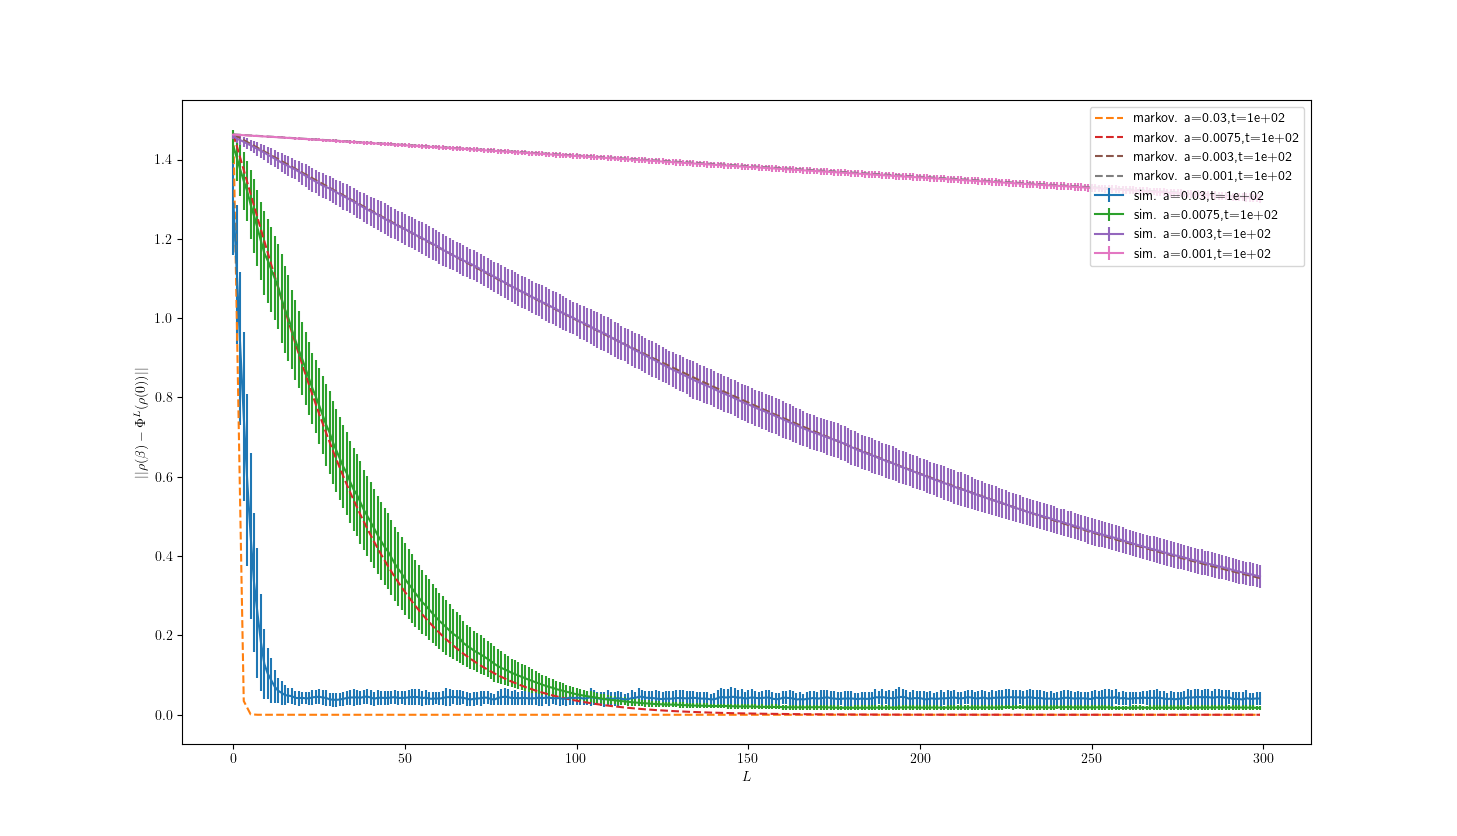
\includegraphics[width=0.45\linewidth]{numerics/data/sho_error_vs_l.png}
    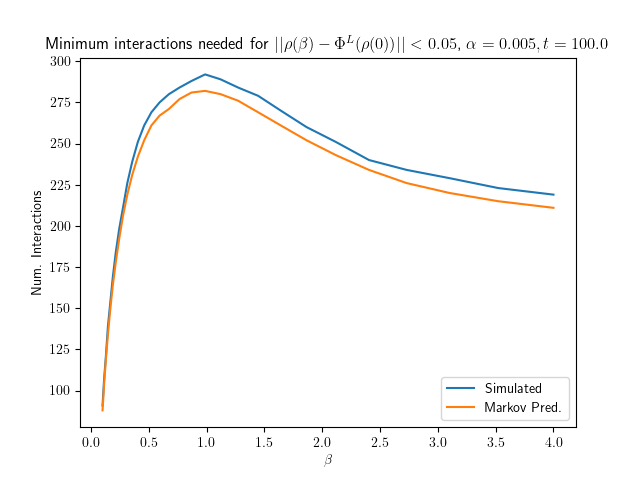
\includegraphics[width=0.45\linewidth]{numerics/data/sho_l_vs_beta.png} \\
    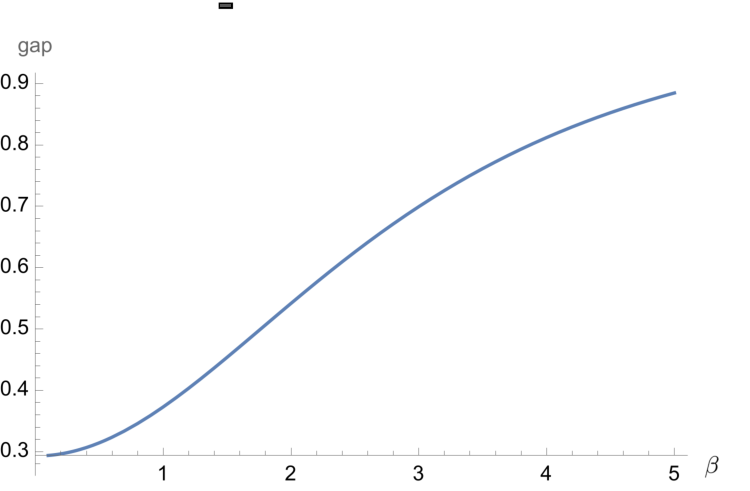
\includegraphics[width=0.5\linewidth]{numerics/data/spec_gap_dim_4.pdf}
    \caption{TODO: Improve. Trace distance to target as a function of interaction number, simulation compared to Markov chain behavior. The Hilbert-Schmidt overlap with the ground state $\anglebrackets{\Phi^L(\rho(0)), \ketbra{0}{0}}$ is 0.940 at $L = 300$. }
    \label{fig:enter-label}
\end{figure}

The behavior of the fixed $\epsilon$ plot reveals a very interesting phenomenon where the number of interactions, and therefore total thermalization time, needed to reach the thermal state goes \emph{down} after a peak at about $\beta = 1.0$. This means colder temperatures can be reached quicker than some intermediate temperatures, assuming a starting state of the maximally mixed state. Our rationale for this behavior is that the spectral gap of the resulting Markov chain must increase with $\beta$ faster than the distance from $\rho(0)$ to $\rho(\beta)$ grows with $\beta$. This bears out when we plot the spectral gap as a function of $\beta$ for the truncated harmonic oscillator, seen in Fig. \ref{fig:enter-label}.

Once we have determined how the thermalization process behaves for a given $\alpha$ and $t$, we can then sweep these parameters to determine how they effect thermalization. From our analysis of the single qubit case we would expect that the distance to the Markov chain can be made arbitrarily close as we both reduce the off-resonant terms by making $\alpha$ smaller and reducing the norm of the remainder terms by making $\widetilde{\alpha}$ smaller. As $t$ is not set we can choose which one to reduce by also varying $t$. As $t$ dictates the simulation time for the system dynamics we would like to reduce it as much as possible. The plot povided in Fig \ref{fig:total_time_vs_time} shows that the total simulation time tends to decrease as $t$ increases until some threshold is met. Finding this optimum value analytically would be intractable for arbitrary dimension harmonic oscillators. One other main takeaway is that as $\alpha$ increases the total simulation time also tends to decrease for a significant range of $t$. This is due to the fact that the probability mass that can be moved by the Markov chain increases with $\alpha$. We did not take this to the extreme and study a strong-coupling, short-time interaction channel and leave these questions for future research. 

\begin{figure}
    \centering
    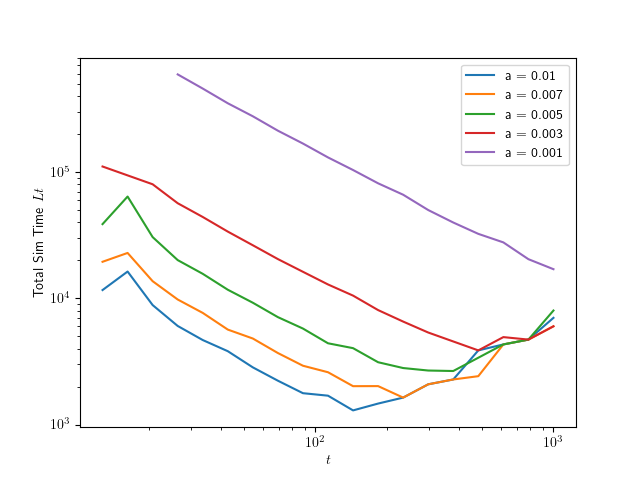
\includegraphics[width=0.75\linewidth]{numerics/data/total_time_vs_time.png}
    \caption{Total simulation time as a function of per-interaction simulation time $t$.}
    \label{fig:total_time_vs_time}
\end{figure}

\section{General Systems}
 Now that we have studied a single qubit and the harmonic oscillator in as much detail as possible, in this section we explore the behavior of our algorithm for some more generic systems. As our algorithm ultimately boils down to a Markov chain over the eigenstates of the Hamiltonian we are unable to make any runtime claims, as that would require bounding the spectral gap of a Markov chain that depends on knowledge of the Hamiltonian eigenvalues. What we do show in this section is three-fold: we first demonstrate that if the environment temperature approaches 0 ($\beta \to \infty$), then the ground state of the system is \emph{a} fixed point, second that if the eigenvalue differences $\lambda(i) - \lambda(j)$ can be sampled from exactly then we show that by taking $t$ sufficiently large the thermal state is the unique fixed point, and lastly we demonstrate that knowledge of eigenvalue gaps is largely an artifact of theory by preparing low temperature thermal states for Hydrogen chains without any a-priori knowledge.
 
% For a generic system it becomes very difficult to make any results without promises about our knowledge of the Hamiltonian. Right away the most obvious problem is that without prior knowledge we have no clue really what value of $\gamma$ we should tune our ancilla qubits to. For the single qubit and harmonic oscillator case we had complete knowledge of the spectrum of $H_S$. One thing we would like to show is that it is possible to do so if we also know the spectrum of $H_S$ completely. This will involve randomly choosing a value of $\gamma$ from the Bohr frequency set with importance sampling. Even with these promises it turns out to be incredibly difficult to analyze the resulting Markov chain for an arbitrary $\beta$. What we will do instead of an arbitrary thermal state preparation is to instead prepare the ground state. As an additional preprocessing step one could apply a filter function like a Heaviside step function to the Hamiltonian, thus eliminating the need for knowledge of eigenvalue gaps. This route was analyzed using Quantum Signal Processing (QSP) techniques in (Cite Danial dynamical cooling). 

We first briefly discuss what happens in the $\beta \to \infty$ limit. In this scenario our ancilla qubit is in the ground state, meaning that any transition that occurs must increase the energy of the ancilla and decrease the energy of the system. Since the ground state is the lowest possible energy, intuitively we would expect that no transitions out of the ground state occur and the ground state should remain fixed. This intuition is captured in the theorem below, where we ignore the effects of controllable off-resonant transitions and order $(\alpha t)^3$ contributions.
\begin{theorem}[Ground State Fixed Point] \label{thm:ground_state_fixed}
    For an arbitrary Hamiltonian $H$ and environment energy gap $\gamma$, in the limit as $\beta \to \infty$ the ground state of $H$ is a fixed point of the on-resonance second order dynamics. Formally,
    \begin{equation}
        \lim_{\beta \to \infty} (\identity + \mathcal{T}_{\on})(\ketbra{0}{0}) = \ketbra{0}{0}.
    \end{equation}
\end{theorem}
\begin{proof}
    To prove this we only have to show that $\lim_{\beta \to \infty} \mathcal{T}_{\on}(\ketbra{0}{0}) = 0$. Suppose $\gamma$ is sufficiently close to the eigenvalue difference $\lambda(j) - \lambda(0)$. Using Eq. \eqref{eq:on_resonance_transitions} from Lemma \ref{thm:on_and_off_resonance} the on-resonance transition amplitude is
    \begin{align}
        \lim_{\beta \to \infty} \bra{j} \mathcal{T}_{\on}(\ketbra{0}{0}) \ket{j} &= \lim_{\beta \to \infty} \widetilde{\alpha}^2 \frac{e^{-\beta \gamma}}{1 + e^{-\beta \gamma}} \sinc^2 \left( \frac{(\Delta(j,0) - \gamma)t}{2} \right) = 0.
    \end{align}
    Since this holds for any $\gamma$ that produces an on-resonance transition we are done.
\end{proof}

Now we move on to showcase a scenario when finite $\beta$ thermal states are the unique fixed point of the Markov dynamics. For this we assume sample access to the eigenvalue differences $\Delta(i,j) = \lambda(i) - \lambda(j)$, meaning if there are $\chi(i,j)$ pairs of eigenvalues with positive differences $\Delta(k,l) = \Delta(i,j) \ge 0$ then the probability we receive $\Delta(i,j)$ is $\prob{\gamma = \Delta(i,j)} = \chi(i,j) \frac{2}{\dim_S(\dim_S - 1)}$. One simplifying assumption we will make (I'm not sure this is necessary?) is that there are no degeneracies in the Hamiltonian and for all $i,j$ we have $\Delta(i,j) > 0$. By taking $t$ larger than the smallest difference between eigenvalue differences we can ensure that the probability of an on-resonance transition occurring between states $i$ and $j$ is $\chi(i,j) \frac{2}{\dim_S(\dim_S - 1)}$. More formally, we use the definition of $\delta_{\min} = \min_{\Delta(k,l) \ge 0 \neq \Delta(i,j)} |\Delta(k,l) - \Delta(i,j)|$ and take $t \ge 1/ \delta_{\min}$ so that we can use Lemma \ref{lem:sinc_poly_approx} to argue that the only contribution to $\bra{j} \mathcal{T}_{\on}(\ketbra{i}{i}) \ket{j}$ is from $\gamma = \Delta(i,j)$. As $\gamma$ is a random variable this makes the transition coefficient a random variable as well, and we will capture this random behavior with an indicator variable. 

\begin{theorem}[Generic System Thermal State Fixed Point]
    Let $H_S$ be an Hermitian matrix with no degenerate eigenvalues, let $\chi(i,j)$ denote the number of eigenvalue differences of value $\Delta(i,j)$, and let $\gamma$ be a random variable with distribution $\prob{\gamma = \Delta(i,j)} = \frac{\chi(i,j)}{\binom{\dim_S}{2}}$. The thermal state $\rho_S(\beta) = \frac{e^{-\beta H_S}}{\partfun(\beta)}$ is the unique fixed point of the Markov chain dynamics of the thermalizing channel $\Phi$ in expectation with respect to $\gamma$, formally
    \begin{align}
        \mathbb{E}_{\gamma} \left[ (\identity + \mathcal{T}_{\on})(\rho_S(\beta)) \right] = \rho_S(\beta).
    \end{align}
    Combined with Jerison's Markov Relaxation Theorem \ref{thm:markov_chain_bound} this implies there exists sufficiently large $L_\star$ and $t$, along with a sufficiently small $\alpha$, such that for all starting states $\rho$ that are diagonal in the $H_S$ basis and for all $\epsilon > 0$
    \begin{equation}
    \norm{\rho_S(\beta) - (\mathbb{E}_\gamma \Phi_\gamma)^{\circ L_\star}(\rho)}_1 \le \epsilon.
    \end{equation}
\end{theorem}

\begin{proof}
For $j > i$ we have $\bra{j} \mathcal{T}_{\on}(\ketbra{i}{i}) \ket{j} = \widetilde{\alpha}^2 q(1; i, j) \mathbf{I}[\gamma = \Delta(i,j)]$ and for $j < i$ we have $\bra{j} \mathcal{T}_{\on}(\ketbra{i}{i}) \ket{j} = \widetilde{\alpha}^2 q(0; i, j) \mathbf{I}[\gamma = \Delta(i,j)]$. 

Now we can compute the expected on-resonance transition over this distribution of $\gamma$ for $i < j$ as
\begin{align}
    \mathbb{E}_{\gamma} \bra{j} \mathcal{T}_{\on}(\ketbra{i}{i}) \ket{j} &= \widetilde{\alpha} \mathbb{E}_{\gamma} q(1; i, j) \mathbf{I}[\gamma = \Delta(i,j)] \\
    &= \widetilde{\alpha}^2 \sum_{k > l} \prob{\gamma = \Delta(k,l)} q(1; i,j) \mathbf{I}[\Gamma = \Delta(i,j)] \\
    &= \widetilde{\alpha}^2 q(1; i,j) \frac{2 \chi(i,j)}{\dim_S(\dim_S - 1)}.
\end{align}
For $ i > j$ the same calculation follows but we replace $q(1; i, j)$ with $q(0;i,j)$ and for $i = j$ we just take the negative sum of all $i \neq j$ . This allows us to calculate the action of $\mathcal{T}_{\on}$ on the thermal state. In order for the thermal state to be a fixed point it must be in the kernel of $\mathcal{T}_{\on}$. To show this we will compute the overlap of the output with the ground state
\begin{align}
    &\mathbb{E}_{\gamma} \bra{0} \mathcal{T}_{\on}(\rho_S(\beta)) \ket{0} \nonumber \\
    &= \frac{1}{\partfun(\beta)} e^{-\beta \lambda(0)} \mathbb{E}_{\gamma} \bra{0} \mathcal{T}_{\on}(\ketbra{0}{0})\ket{0} + \frac{1}{\partfun(\beta)} \sum_{j > 0} e^{-\beta \lambda(j)} \mathbb{E}_{\gamma}  \bra{0} \mathcal{T}_{\on}(\ketbra{j}{j}) \ket{0} \\
    &= \frac{-1}{\partfun(\beta)} e^{-\beta \lambda(0)} \sum_{k > 0} \mathbb{E}_{\gamma} \bra{k} \mathcal{T}_{\on}(\ketbra{0}{0}) \ket{k} + \frac{1}{\partfun(\beta)} \sum_{j > 0} e^{-\beta \lambda(j)} \widetilde{\alpha}^2 q(0; 0, j) \frac{2 \chi(i,j)}{\dim_S (\dim_S - 1)} \\
    &= \frac{-1}{\partfun(\beta)} e^{-\beta \lambda(0)} \sum_{k > 0} \widetilde{\alpha}^2 q(1; 0, k) \frac{2 \chi(0, k)}{\dim_S(\dim_S - 1)} + \frac{1}{\partfun(\beta)} \sum_{j > 0} \widetilde{\alpha}^2 \frac{e^{-\beta \lambda(j)} }{1 + e^{-\beta \Delta(j, 0)}} \frac{2 \chi(0,j)}{\dim_S (\dim_S - 1)} \\
    &= \frac{2 \widetilde{\alpha}^2}{\partfun(\beta) \dim_S(\dim_S - 1)} \left(-\sum_{k > 0} e^{-\beta \lambda(0)} \frac{e^{-\beta \Delta(k, 0)}}{1 + e^{-\beta \Delta(k,0)}} \chi(0, k) + \sum_{j > 0} \frac{e^{-\beta \lambda(j)}}{1 + e^{-\beta \Delta(j, 0)}} \chi(0, j) \right) \\
    &= 0,
\end{align}
where we note that $e^{-\beta \lambda(0)} e^{-\beta \Delta(k, 0)} = e^{-\beta \lambda(k)}$ and we simply relabel the left summation index $k \mapsto j$, which then cancels with the other sum giving 0.

We now repeat the above calculation for the transition amplitude to the states in the middle with $0 < j < \dim_S - 1$. The main difference with this calculation is that we now have to split our summation into states with higher or lower energy than the input states. 
\begin{align}
    &\mathbb{E}_{\gamma} \bra{j} \mathcal{T}_{\on}(\rho_S(\beta)) \ket{j} \nonumber \\
    &= \frac{1}{\partfun(\beta)} \sum_{k < j} e^{-\beta \lambda(k)} \mathbb{E}_{\gamma} \bra{j} \mathcal{T}_{\on}(\ketbra{k}{k}) \ket{j} + \frac{e^{-\beta \lambda(j)}}{\partfun(\beta)} \mathbb{E}_{\gamma}\bra{j} \mathcal{T}_{\on} (\ketbra{j}{j}) \ket{j} + \frac{1}{\partfun(\beta)} \sum_{k > j} e^{-\beta \lambda(k)} \mathbb{E}_{\gamma} \bra{j} \mathcal{T}_{\on} (\ketbra{k}{k}) \ket{j}. \label{eq:generic_system_fixed_point_1}
\end{align}
We then can break down the middle self-transition term as the negative sum over the other transition elements as
\begin{align}
    \frac{e^{-\beta \lambda(j)}}{\partfun(\beta)} \mathbb{E}_{\gamma}\bra{j} \mathcal{T}_{\on} (\ketbra{j}{j}) \ket{j} &= - \frac{e^{-\beta \lambda(j)}}{\partfun(\beta)} \sum_{l < j} \mathbb{E}_{\gamma} \bra{l} \mathcal{T}_{\on} (\ketbra{j}{j}) \ket{l} - \frac{e^{-\beta \lambda(j)}}{\partfun(\beta)} \sum_{l > j} \mathbb{E}_{\gamma} \bra{l} \mathcal{T}_{\on} (\ketbra{j}{j}) \ket{l} \\
    &= -  \frac{2 \widetilde{\alpha}^2 e^{-\beta \lambda(j)} }{\partfun(\beta) \dim_S(\dim_S - 1)} \left( \sum_{l < j} q(0; l, j) \chi(l, j) + \sum_{l > j} q(1; l, j) \chi(l, j) \right) \\
    &= -  \frac{2 \widetilde{\alpha}^2  }{\partfun(\beta) \dim_S(\dim_S - 1)} \left( \sum_{l < j} \frac{e^{-\beta \lambda(j)}}{1 + e^{-\beta \Delta(j, l)}} \chi(l, j) + \sum_{l > j} \frac{e^{-\beta \lambda(l)}}{1 + e^{-\beta \Delta(l, j)}} \chi(l, j) \right). \label{eq:generic_system_fixed_point_2}
\end{align}
Now we can return to Eq. \eqref{eq:generic_system_fixed_point_1} and compute the expectation values within the sums as
\begin{align}
    \frac{1}{\partfun(\beta)} \sum_{k < j} e^{-\beta \lambda(k)} \mathbb{E}_{\gamma} \bra{j} \mathcal{T}_{\on}(\ketbra{k}{k}) \ket{j} &= \frac{2 \widetilde{\alpha}^2 }{\partfun(\beta) \dim_S(\dim_S - 1) } \sum_{k < j} e^{-\beta \lambda(k)} \frac{e^{-\beta \Delta(j, k)}}{1 + e^{-\beta \Delta(j, k)}} \chi(j, k) \\
    &= \frac{2 \widetilde{\alpha}^2 }{\partfun(\beta) \dim_S(\dim_S - 1) } \sum_{k < j} \frac{e^{-\beta \lambda(j)}}{1 + e^{-\beta \Delta(j, k)}} \chi(j, k), \label{eq:generic_system_fixed_point_3}
\end{align}
and likewise
\begin{align}
    \frac{1}{\partfun(\beta)} \sum_{k > j} e^{-\beta \lambda(k)} \mathbb{E}_{\gamma} \bra{j} \mathcal{T}_{\on}(\ketbra{k}{k}) \ket{j} &= \frac{2 \widetilde{\alpha}^2 }{\partfun(\beta) \dim_S(\dim_S - 1) } \sum_{k < j} e^{-\beta \lambda(k)} \frac{1}{1 + e^{-\beta \Delta(k, j)}} \chi(j, k). \label{eq:generic_system_fixed_point_4}
\end{align}
After relabeling summation indices, it is clear that adding Eqs. \eqref{eq:generic_system_fixed_point_2}, \eqref{eq:generic_system_fixed_point_3}, and \eqref{eq:generic_system_fixed_point_4} is equal to \eqref{eq:generic_system_fixed_point_1} and that therefore $0 < j < \dim_S - 1 \implies \bra{j} \mathcal{T}_{\on}(\rho_S(\beta)) \ket{j} = 0$.

To prove that the final transition amplitude is 0 we can use the fact that the trace of the on-resonance map is 0
\begin{align}
    \trace{\mathcal{T}_{\on}(\rho_S(\beta))} &= \sum_j \bra{j} \mathcal{T}_{\on}(\rho_S(\beta)) \ket{j} = 0\\
    \implies \bra{\dim_S - 1} \mathcal{T}_{\on}(\rho_S(\beta)) \ket{\dim_S - 1} &= - \sum_{j < \dim_S - 1} \bra{j} \mathcal{T}_{\on}(\rho_S(\beta)) \ket{j} \\ 
    &= 0.
\end{align}
This completes the proof that $\rho_S(\beta)$ is a fixed point of $\identity + \mathbb{E}_{\gamma} \mathcal{T}_{\on}$. To see that it is the unique fixed point we need to show ergodicity of the Markov chain $I + T$. The condition of ergodicity requires that the expected hitting time of any target state $j$ from any initial state $i$ is finite. Given our assumption of sample access to the $\Delta(i,j)$ distribution we have 
\begin{align}
    \bra{j} (\identity + \mathbb{E}_{\gamma} \mathcal{T}_{\on})(\ketbra{i}{i}) \ket{j} &= |\braket{j}{i}|^2 + \mathbb{E}_{\gamma} \bra{j} \mathcal{T}_{\on} (\ketbra{i}{i}) \ket{j}.
\end{align}
If $i = j$ the result is on the order of $1 - \Theta(\widetilde{\alpha}^2 \frac{2}{\dim_S (\dim_S - 1)})$, which approaches 1 as $\widetilde{\alpha} \to 0$, and is clearly greater than zero. If $i < j$ the result is $\frac{2 \widetilde{\alpha}^2}{\dim_S (\dim_S - 1)} q(1; i,j) \chi(i,j)$ which is positive. If $i > j$ the result is $\frac{2 \widetilde{\alpha}^2}{\dim_S (\dim_S - 1)} q(0; i,j) \chi(i,j)$ which again is positive. These three results show that for all $i$ and $j$ there is a nonzero probability of transitioning from $i$ to $j$ within a single interaction, thereby showing ergodicity. As $\norm{\mathcal{T}_{\off}}_1 \le \frac{4 \alpha^2}{\delta_{\min}^2}$ and $\norm{R_{\Phi}}_1 \in \bigo{\alpha^3 t^3}$ there exists a small enough value of $\alpha$ such that $L_{\star}(\norm{\mathcal{T}_{\off}}_1 + \norm{R_{\Phi}}_1) \le \epsilon / 2$. The Markov Relaxation Theorem \ref{thm:markov_chain_bound} tells us that taking $L_{\star}$ sufficiently large yields $\norm{\rho_S(\beta) + (\identity + \mathbb{E}_{\gamma} \mathcal{T}_{\on})^{\circ L_{\star}}(\rho)}_1 \le \epsilon /2$. This completes the proof.
\end{proof}

One of the main drawbacks to our results thus far has been that the runtime depends on the spectral gap of a Markov chain, which in turn varies based on our knowledge of the eigenvalue differences $\Delta_S(i,j)$. Although characterizing this dependency analytically seems incredibly difficult, it is rather straightforward to test how well it works numerically on small, classically simulable systems. We did just this for two Hydrogen chain systems, H2 and H3, which are a standard benchmark system in computational chemistry. For each interaction we sample a value of $\gamma$ from a Gaussian distribution with mean $\trace{H_S}$ and variance $\frac{|\norm{H_S} - \trace{H_S}}{2}$, the trace is relatively easy to compute and $\norm{H_S}$ can typically be upper bounded. We then tracked the distance of the system state with each interaction and see a decrease in the error as the number of interactions proceeds. We observe that this rather oblivious distribution of $\gamma$ leads to surprisingly good results for conservative values of $\alpha = 10^{-3}$ and $t = 10^2$; we achieve a trace distance of 0.06 to the thermal state for $\beta = 3$ for H2 and $0.1$ for H3. 

 We report on numeric investigations on the performance of this algorithm for simple Hydrogen chain systems, a common benchmarking system for the performance of quantum chemistry algorithms. We will run a basic implementation of this algorithm, using exact matrix exponentiation to implement the time evolution operators $e^{\pm i (H_S + H_E + \alpha G)t}$ and measure the trace distance to the exact thermal state, also computed using matrix exponentiation. We will use rather conservative choices of $\alpha = 0.001$ and $t = 100.0$ for all hydrogen chains. To choose $\gamma$ we will sample a value randomly from a Gaussian random variable centered at the average eigenvalue of $H_S$, computed using the trace identity $\trace{H_S} = \sum \lambda(i)$ and divide by the dimension of the Hilbert space. 

\bibliographystyle{unsrt}
\bibliography{bib}

\appendix



\section{Sinc Function}

\begin{lemma}[Sinc Function Bounds] \label{lem:sinc_poly_approx}
    For $\sinc^2\left( \frac{x t}{2} \right)$ and $\delta_{\min} \coloneqq \min_{\Delta(i,j) \neq \Delta(k,l)} \left| \Delta(i,j) - \Delta(k, l) \right|$, we will make significant use of the following bounds:
    \begin{align}
        |x| \ge \delta_{\min} &\implies \sinc^2 \left( \frac{x t}{2} \right) \le \frac{4}{\delta_{\min}^2 t^2} \label{eq:sinc_upper_bound} \\
        |x| \le  \frac{2 \sqrt{2}}{\delta_{\min} t^2} &\implies \sinc^2\left(\frac{x t}{2} \right) \ge 1 - \frac{4}{\delta_{\min}^2 t^2}. \label{eq:sinc_lower_bound}
\end{align}

\end{lemma}
\begin{proof}
    The first inequality is rather trivial
    \begin{align}
        \sinc^2 \left( \frac{x t}{2} \right) &= \frac{\sin^2 (x t /2)}{(x t / 2)^2} \le \frac{4}{x^2 t^2} \le \frac{4}{\delta_{\min}^2 t^2}.
    \end{align}
    The second involves a Taylor Series for $\sinc^2$, which we compute using the expression of $\sinc$ as $\sinc(x t/ 2) = \frac{\sin xt /2}{xt/2} = \int_0^1 \cos(sxt/2) ds$.  The first two derivatives can then be computed straightforwardly by noting that the derivative can be pulled into the integral by the Liebniz integral rule
    \begin{align}
        \frac{d \sinc^2(x t /2)}{dx} &= - t \int_0^1 \sin(sx) s ds \int_0^1 \cos(sx) ds \\
        \frac{d^2 \sinc^2(x t /2)}{dx^2} &= -t^2 / 2 \int_0^1 \cos(sx)s^2 ds \int_0^1 \cos(sx) ds + t^2 / 2 \int_0^1 \sin(sx) s ~ds \int_0^1 \sin(sx) s ~ds.
    \end{align}
    We can evaluate each of these derivatives about the origin using continuity of the derivatives along with the limits $\lim_{x \to 0} \cos(sx) = 1$ and $\lim_{x \to 0} \sin(sx) = 0$. We can now compute the mean-value version Taylor series as
    \begin{align}
        \sinc^2 \left(\frac{x t}{2} \right) &= \sinc^2(0) + x \frac{d}{dx} \sinc^2 \left(\frac{x t}{2} \right) \bigg|_{x = 0} + \frac{x^2}{2!} \frac{d^2}{dx^2} \sinc^2 \left(\frac{x t}{2} \right) \bigg|_{x = x_{\star}},
    \end{align}
    where $x_{\star} \in [0,1]$. 
    Plugging in $\sinc^2(0) = 1$ and $\frac{d\sinc^2(x t /2)}{dx}\big|_{x = 0} = 0$ then yields $|\sinc^2(xt/2) - 1| = \frac{|x|^2}{2} \abs{\frac{d^2\sinc^2(x t / 2)}{dx^2}\big|_{x = x_{\star}}}$. We make use of the rather simplistic bound
    \begin{align}
        \abs{\frac{d^2\sinc^2(sxt/2)}{dx^2}\bigg|_{x = x_{\star}} } &\leq t^2 / 2 \abs{\int_0^1 \cos(sx_{\star} t/ 2) s^2 ds \int_0^1 \cos(sx_{\star} t/ 2) ds} + t^2 /2 \abs{\int_0^1 \sin(sx_{\star} t/ 2) s ds \int_0^1 \sin(sx_{\star} t/ 2) s ds} \\
        &\leq t^2 / 2 \int_0^1 \abs{\cos(sx_{\star} t/2)} s^2 ds \int_0^1 \abs{\cos(sx_{\star} t /2 )} ds + t^2 / 2 \parens{\int_0^1 \abs{\sin(sx_{\star} t /2)} |s| ds}^2 \\
        &\leq t^2 / 2 \int_0^1 s^2 ds + t^2 / 2 \parens{\int_0^1 s ds}^2 \\
        &\leq t^2.
    \end{align}
    This yields the final inequality $|\sinc^2(x t /2 ) - 1| \leq \frac{|x|^2 t^2}{2}$. Requiring $|x| \le  \frac{2 \sqrt{2}}{\delta_{\min} t^2}$ yields Eq. \eqref{eq:sinc_lower_bound}.
\end{proof}


\section{Haar Integral Proofs} \label{sec:haar_integral_appendix}

In this section we present the more technical work needed to state our results in Section \ref{sec:taylor_series_phi}. The first two results are Lemmas that compute the effects of the randomized interaction in a form that are usable in the main result of Theorem \ref{lem:big_one}.

\begin{lemma} \label{lem:two_heisenberg_interactions}
    Let $G(t)$ denote the Heisenberg evolved random interaction $G(t) = e^{iHt} G e^{-iHt}$ for a total Hamiltonian $H$. After averaging over the interaction measure the product $G(x) G(y)$ can be computed as
    \begin{equation}
        \int G(x) G(y) dG = \frac{1}{\dim + 1} \parens{\sum_{(i,j),(k,l)} e^{i \Delta(i,j|k,l) (x-y)} \ketbra{i,j}{i,j} + \identity}.
    \end{equation}
\end{lemma}
\begin{proof}
The overall structure of this proof is to evaluate the product in the Hamiltonian eigenbasis and split the product into three factors: a phase contribution from the time evolution, a Haar integral from the eigenvalues of the random interaction, and the eigenvalue contribution of the random interaction. Since this involves the use of multiple indices, it will greatly simplify the proof to use a single index over the total Hilbert space $\hilb$ as opposed to two indices over $\hilb_S \otimes \hilb_E$. For example, the index $a$ should be thought of as a pair $(a_s, a_e)$, and functions $\lambda(a)$ should be thought of as $\lambda(a_s, a_e)$. Once the final form of the expression is reached we will substitute in pairs of indices for easier use of the lemma in other places.
    \begin{align}
        \int G(x) G(y) dG &= \int e^{+i H x} U_G D U_G^\dagger e^{-i H x} e^{+i H y} U_G D U_G^\dagger e^{-i H y} dU_G ~dD \\
        &= \int \bigg[\sum_a e^{+i \lambda(a)x}\ketbra{a}{a}  U_G \sum_b D(b)\ketbra{b}{b} U_G^\dagger \nonumber \\
        &\quad \sum_c e^{-i \lambda(c) (x - y)} \ketbra{c}{c} U_G \sum_d D(d)\ketbra{d}{d} U_G^\dagger \sum_e e^{-i \lambda(e) y} \ketbra{e}{e} \bigg] dU_G ~dD\\
        &=\sum_{a,b,c,d,e} \ketbra{a}{e} e^{-i (\lambda(c) - \lambda(a))x} e^{-i (\lambda(e) - \lambda(c))y} \nonumber \\
        &\quad \times \int \bra{a} U_G \ket{b} \bra{c} U_G \ket{d} \bra{b} U_G^{\dagger} \ket{c} \bra{d} U_G^\dagger \ket{e} dU_G \int D(b) D(d) dD \\
        &=  \sum_{a, b, c, d, e} \delta_{bd} \ketbra{a}{e} e^{-i (\lambda(c) - \lambda(a))x} e^{-i (\lambda(e) - \lambda(c))y} \nonumber \\
        &\quad \times \int \bra{a} U_G \ket{b} \bra{c} U_G \ket{d} \bra{b} U_G^{\dagger} \ket{c} \bra{d} U_G^\dagger \ket{e} dU_G. \\
    \end{align}
    Now the summation over $d$ fixes $d=b$ and we use Lemma \ref{lem:haar_two_moment} to compute the Haar integral, which simplifies greatly due to the repeated $b$ index. Plugging the result into the above yields the following
    \begin{align}
        &= \frac{1}{\dim^2 - 1} \sum_{a, b, c, e} \ketbra{a}{e} e^{-i (\lambda(c) - \lambda(a))x} e^{-i (\lambda(e) - \lambda(c))y} \parens{\delta_{ac} \delta_{ce} + \delta_{ae} - \frac{1}{\dim} \parens{\delta_{ac} \delta_{ce} + \delta_{ae}}}  \\
        &= \frac{1}{\dim^2 - 1} \parens{1 - \frac{1}{\dim}} \sum_{a, b, c, e} \ketbra{a}{e} e^{-i (\lambda(c) - \lambda(a))x} e^{-i (\lambda(e) - \lambda(c))y} \delta_{ae} (1 + \delta_{ac}) \\
        &= \frac{1}{\dim^2 - 1} \parens{1 - \frac{1}{\dim}} \sum_{a, b, c} \ketbra{a}{a} e^{i (\lambda(a) - \lambda(c))(x-y)} (1 + \delta_{ac}) \\
        &= \frac{1 \parens{\dim - 1}}{\dim^2 - 1} \sum_{a,c} \ketbra{a}{a} e^{i (\lambda(a) - \lambda(c))(x - y)} (1 + \delta_{ac}) \\
        &= \frac{1}{\dim + 1} \parens{\sum_{a,c} e^{i (\lambda(a) - \lambda(c))(x-y)} \ketbra{a}{a} + \identity}.
    \end{align}
    Reindexing by $a \mapsto i,j$, $c \mapsto k,l$, and plugging in the definition of $\Delta$ yields the statement of the lemma.
\end{proof}


\begin{lemma} \label{lem:sandwiched_interaction}
    Given two Heisenberg evolved random interactions, $G(x)$ and $G(y)$, we compute their action on an outer-product $\ketbra{i,j}{k,l}$ as
    \begin{equation}
        \int G(x) \ketbra{i,j}{k,l} G(y) ~dG = \frac{1}{\dim + 1} \parens{\ketbra{i,j}{k,l} + \delta(i,j|k,l) \sum_{m,n} e^{i \Delta(m,n | i,j) (x-y)} \ketbra{m,n}{m,n}}
    \end{equation}
\end{lemma}
\begin{proof}
This proof is structured the same as Lemma \ref{lem:two_heisenberg_interactions} and similarly we will use a single index of the total Hilbert space $\hilb$ and switch to two indices to match the rest of the exposition.
    \begin{align}
        \int G(x) \ketbra{a}{b} G(y) dG &=  \int e^{i H x} U_G D U_G^{\dagger} e^{-i H x} \ketbra{a}{b} e^{i H y} U_G D U_G^\dagger e^{-i H y} ~dG \\
        &= \sum_{c, d, e, f} e^{i (\lambda(c) - \lambda(a))x} e^{i (\lambda(b) - \lambda(f))y} \nonumber \\
        &\quad \times \int \ketbra{c}{c} U_G D(d) \ketbra{d}{d} U_G^\dagger \ketbra{a}{b} U_G D(e) \ketbra{e}{e} U_G^\dagger \ketbra{f}{f} dG \\
        &= \sum_{c, d, e, f}  e^{i (\lambda(c) - \lambda(a))x} e^{i (\lambda(b) - \lambda(f))y} \ketbra{c}{f} \nonumber \\
        &\quad \times \int D(d) D(e) dD \int \bra{c} U_G \ket{d} \bra{b} U_G \ket{e} \bra{d} U_G^\dagger \ket{a} \bra{e} U_G^\dagger \ket{f} dU_G \\
        &=  \sum_{c,d,f} e^{i (\lambda(c) - \lambda(a))x} e^{i (\lambda(b) - \lambda(f))y} \ketbra{c}{f} \nonumber \\ 
        &\quad \times \int \bra{c} U_G \ket{d} \bra{b} U_G \ket{d} \bra{a} \overline{U_G} \ket{d} \bra{f} \overline{U_G} \ket{d} dU_G \\
        &= \frac{1}{\dim^2 - 1} \sum_{c,d,f} e^{i (\lambda(c) - \lambda(a))x} e^{i (\lambda(b) - \lambda(f))y} \ketbra{c}{f} (\delta_{ca} \delta_{bf} + \delta_{cf}\delta_{ab})\parens{1 - \frac{1}{\dim}} \\
        &= \frac{1}{\dim + 1} \sum_{c,f} e^{i (\lambda(c) - \lambda(a))x} e^{i (\lambda(b) - \lambda(f))y} \ketbra{c}{f} (\delta_{ca} \delta_{bf} + \delta_{cf}\delta_{ab}) \\
        &= \frac{1}{\dim + 1} \parens{\ketbra{a}{b} + \delta_{ab} \sum_{c} e^{i(\lambda(c) - \lambda(a))(x-y)} \ketbra{c}{c} }.
    \end{align}
    Now re-indexing by $a \mapsto (i,j)$, $b \mapsto (k,l)$ and $c \mapsto (m,n)$ results in the expression given in the statement of the lemma.
\end{proof}


\secondOrderChannelHaar*
\begin{proof}
To start we would like to note that we will use a single index notation to refer to the joint system-environment eigenbasis during this proof to help shorten the already lengthy expressions. We will convert back to a double index notation to match the statement of the theorem. We start from the expression for the first derivative of the channel $\frac{\partial}{\partial \alpha} \Phi_G(\rho_S)$ given by Eq. \eqref{eq:first_order_alpha_derivative}. To take the second derivative there are six factors involving $\alpha$, so we will end up with six terms. We repeat Eq. \eqref{eq:first_order_alpha_derivative} below, add a derivative, and label each factor containing an $\alpha$ for easier computation
\begin{align}
    \frac{\partial^2}{\partial \alpha^2} \Phi_G(\rho_S) =& \frac{\partial}{\partial \alpha} \parens{\int_{0}^{1} \underset{\substack{\downarrow \\ (A)}}{e^{i s (H+\alpha G)t}} (i t G) \underset{\substack{\downarrow \\ (B)}}{e^{i (1-s) (H+\alpha G)t}} ds ~ \rho \underset{\substack{\downarrow \\ (C)}}{e^{-i(H+\alpha G)t}} } \nonumber \\
    &~ ~+\frac{\partial}{\partial \alpha} \parens{ \underset{\substack{\downarrow \\ (D)} }{e^{i(H+\alpha G)t}} \rho \int_{0}^1 \underset{\substack{\downarrow \\ (E)} }{e^{-i s (H+\alpha G) t} } (- i t G) \underset{\substack{\downarrow \\ (F)}}{e^{-i (1-s) (H+\alpha G)t}} ds }. \label{eq:second_derivative_labels}
\end{align}
Our goal is to get each of these terms in a form in which we can use either Lemma \ref{lem:two_heisenberg_interactions} or \ref{lem:sandwiched_interaction}. 
\begin{align}
    (A) &=i t\int_0^1 \parens{\frac{\partial}{\partial \alpha} e^{i s_1 (H+ \alpha G)t}} G e^{i(1-s_1)(H+\alpha G)t} ds_1 \rho e^{-i (H+\alpha G)t} \bigg|_{\alpha=0} \\
    &= (it)^2 \int_0^1 \parens{\int_0^1 e^{i s_1 s_2 (H+\alpha G)t} s_1 G e^{i s_1 (1-s_2) (H+\alpha G)t} ds_2} G e^{i(1-s_1) (H+\alpha G)t} ds_1 \rho e^{-i(H+\alpha G) t} \bigg|_{\alpha=0} \label{eq:second_order_deriv_intermediate_a}\\
    &= -t^2 \int_0^1 \int_0^1 e^{i s_1 s_2 H t} G e^{-i s_1 s_2 H t} e^{i s_1 H t} G e^{-i s_1 H t} s_1 ds_1 ds_2 e^{i H t} \rho e^{-i H t} \\
    &= -t^2 \int_0^1 \int_0^1 G(s_1 s_2 t) G(s_1 t) s_1 ds_1 ds_2 \rho(t). \label{eq:second_deriv_alpha_first_term}
\end{align}

\begin{align}
    (B) &= it \int_0^1 e^{i s_1 (H + \alpha G)t} G \frac{\partial}{\partial \alpha}\parens{e^{i(1-s_1)(H + \alpha G)t}} ds_1 \rho e^{-i(H + \alpha G) t} \bigg|_{\alpha = 0} \\
    &= (it)^2 \int_0^1 e^{i s_1 (H + \alpha G)t} G \parens{\int_0^1 e^{i(1-s_1)s_2 (H + \alpha G)t} (1-s_1) G e^{i(1 - s_1)(1 - s_2)(H + \alpha G)t} ds_2} ds_1 ~ \rho e^{-i ( H + \alpha G)t} \bigg|_{\alpha = 0} \\
    &= -t^2 \int_0^1 \int_0^1 e^{i s_1 H t} G e^{i(1-s_1)s_2 H t} G e^{i(1-s_1)(1-s_2) H t} (1-s_1) ds_1 ds_2 ~ \rho e^{-i H t}\\ 
    &= -t^2 \int_0^1 \int_0^1 e^{i s_1 H t} G e^{-i s_1 H t} e^{i(s_1 + s_2 - s_1 s_2) H t} G e^{-i (s_1 + s_2 - s_1 s_2) H t} (1-s_1) ds_1 ds_2 ~ \rho(t) \\
    &= -t^2 \int_0^1 \int_0^1 G(s_1 t) G((s_1 + s_2 - s_1 s_2)t) (1-s_1) ds_1 ds_2 ~ \rho(t)
\end{align}

\begin{align}
    (C) &= it \int_0^1 e^{i s (H + \alpha G)t} G e^{i(1-s) (H + \alpha G) t} ds ~\rho ~ \frac{\partial}{\partial \alpha} \parens{ e^{-i (H + \alpha G) t} } \bigg|_{\alpha = 0} \\
    &= (i t) (-it) \int_0^1 e^{i s (H + \alpha G)t} G e^{i (1 - s) (H + \alpha G)t} ds ~ \rho ~ \parens{ \int_0^1 e^{-i s (H + \alpha G)t} G e^{-i (1- s) ( H + \alpha G)t } ds}\bigg|_{\alpha = 0} \\
    &= + t^2 \parens{\int_0^1 e^{i s H t} G e^{-i s H t} ds} e^{i H t} \rho e^{-i H t} \parens{\int_0^1 e^{i (1-s) H t} G e^{-i (1-s) H t} ds} \\
    &= + t^2 \int_0^1 G(st) ds ~ \rho(t) \int_0^1 G((1-s)t) ds
\end{align}

\begin{align}
    (D) &= (-it) \frac{\partial}{\partial \alpha} \parens{e^{i(H + \alpha G)t}} \rho \int_0^1 e^{-i s (H + \alpha G)t} G e^{-i (1-s)(H + \alpha G)t} ds \bigg|_{\alpha = 0} \\
    &= t^2 \parens{\int_0^1 e^{i s (H+ \alpha G)t} G e^{i (1-s) (H + \alpha G)t}ds} \rho \int_0^1 e^{-i s (H + \alpha G)t} G e^{-i (1-s)(H + \alpha G)t} ds \bigg|_{\alpha = 0} \\
    &=  t^2 \int_0^1 e^{i s H t} G e^{-i s H t} ds ~\rho(t) \int_0^1 e^{i (1-s) H t} G e^{-i (1-s) H t} ds \\
    &= t^2 \int_0^1 G(st) ds ~ \rho(t) ~ \int_0^1 G((1-s)t) ds
\end{align}

\begin{align}
    (E) &= (-it) e^{i (H+ \alpha G) t} ~ \rho ~\int_0^1 \frac{\partial}{\partial \alpha} \parens{e^{-i s_1 (H + \alpha G)t}} G e^{-i (1-s_1)(H + \alpha G)t} ds_1 \bigg|_{\alpha = 0} \\
    &= - t^2 e^{i(H + \alpha G)t} ~ \rho ~\int_0^1 \parens{\int_0^1 e^{-i s_1 s_2 (H + \alpha G) t} (s_1 G) e^{-i s_1 (1-s_2) (H + \alpha G)t} ds_2} G e^{-i(1-s_1)(H + \alpha G)t} ds_1 \bigg|_{\alpha = 0} \\
    &= -t^2 e^{i H t} \rho e^{-i H t} \int_0^1 \int_0^1 e^{i (1 - s_1 s_2) H t} G e^{-i (s_1 - s_1 s_2)H t} G e^{-i (1-s_1)H t} s_1 ds_1 ds_2 \\
    &= -t^2 \rho(t) \int_0^1 \int_0^1 G((1- s_1 s_2) t) G((1-s_1)t) s_1 ds_1 ds_2
\end{align}

\begin{align}
    (F) &= (-it) e^{i(H + \alpha G) t} \rho \int_0^1 e^{-i s_1 ( H + \alpha G) t} G \frac{\partial}{\partial \alpha} \parens{ e^{-i (1-s_1) ( H +\alpha G)t}} ds_1 \bigg|_{\alpha = 0} \\
    &= (-it)^2 e^{i (H + \alpha G)t} \rho \int_0^1 e^{-i s_1 (H + \alpha G)t} G \parens{\int_0^1 e^{-i(1-s_1) s_2 (H + \alpha G)t} (1-s_1) G e^{-i(1-s_1) (1-s_2) (H + \alpha G) t} ds_2} ds_1 \bigg|_{\alpha = 0} \\
    &= -t^2 e^{-i H t} \rho e^{-i H t} \int_0^1 \int_0^1 e^{i (1- s_1) H t} G e^{-i (1-s_1) H t} e^{i (1-s_1)(1-s_2) H t} G e^{-i(1-s_1)(1-s_2) H t} (1-s_1) ds_1 ds_2 \\
    &= -t^2 \rho(t) \int_0^1 \int_0^1 G((1-s_1)t) G((1-s_1)(1 - s_2) t) (1-s_1)ds_1 ds_2
\end{align}

Now our goal is to compute the effects of averaging over the interaction $G$ on the above terms, starting with $(A)$. As this involves a lot of index manipulations, similarly to the proofs of Lemmas \ref{lem:two_heisenberg_interactions} and \ref{lem:sandwiched_interaction} we will use a single index for the total system-environment Hilbert space and switch back to a double index to state the results. We will make heavy use of Lemma \ref{lem:two_heisenberg_interactions}.
\begin{align}
    \int (A) dG &= -t^2 \int_0^1 \int_0^1 \int G(s_1 s_2 t) G(s_1 t) dG s_1 ds_1 ds_2 \rho(t) \\
    &= \frac{-t^2 }{\dim + 1} \int_0^1 \int_0^1 \parens{\sum_{i,j} e^{i (\lambda(i) - \lambda(j)) (s_1 s_2 t - s_1 t)} \ketbra{i}{i} + \identity} s_1 ds_1 ds_2 \rho(t) \\
    &= \frac{- t^2 }{\dim + 1} \parens{\sum_{i} \sum_{j : \lambda(i) \neq \lambda(j)} \int_0^1 \int_0^1 e^{i(\lambda(i) - \lambda(j))t (s_1 s_2 - s_1)} s_1 ds_1 ds_2 \ketbra{i}{i} + \sum_{i} \sum_{j : \lambda(i) = \lambda(j)}\frac{1}{2} \ketbra{i}{i} + \frac{1}{2} \identity} \rho(t) \\
    &= \frac{- t^2 }{\dim + 1} \parens{\sum_i \sum_{j : \lambda(i) \neq \lambda(j)} \frac{1 - i (\lambda(i) - \lambda(j))t - e^{-i (\lambda(i) - \lambda(j))t}}{t^2 (\lambda(i) - \lambda(j))^2} \ketbra{i}{i} + \frac{1}{2} \sum_{i} (\eta(i) + 1) \ketbra{i}{i} } \rho(t) \\
    &= \frac{- 1}{\dim + 1}\parens{\sum_{i} \sum_{j: \Delta_{ij} \neq 0} \frac{1 - i \Delta_{ij}t - e^{-i \Delta_{ij} t}}{\Delta_{ij}^2} \ketbra{i}{i} + \frac{t^2}{2} \sum_{i} (\eta(i) + 1)\ketbra{i}{i} } \rho(t)
\end{align}

We can similarly compute the averaged $(B)$ term:
\begin{align}
    \int (B) dG &= -t^2 \int_0^1 \int_0^1 \int G(s_1 t) G((s_1 + s_2 - s_1 s_2) t) dG (1-s_1) ds_1 ds_2 ~ \rho(t) \\
    &= \frac{- t^2 }{\dim + 1} \int_0^1 \int_0^1 \parens{\sum_{i,j} e^{i (\lambda(i) - \lambda(j))(s_1 s_2 - s_2) t} \ketbra{i}{i} + \identity} (1 -s_1) ds_1 ds_2 \rho \\
    &= \frac{- t^2 }{\dim + 1} \parens{\sum_{i} \sum_{j : \lambda(i) \neq \lambda(j)} \int_0^1 \int_0^1 e^{i(\lambda(i) - \lambda(j))t (s_1 s_2 - s_2)} (1 - s_1) ds_1 ds_2 \ketbra{i}{i} + \sum_{i} \sum_{j : \lambda(i) = \lambda(j)}\frac{1}{2} \ketbra{i}{i} + \frac{1}{2} \identity} \rho(t) \\
    &= \frac{- t^2 }{\dim + 1} \parens{\sum_i \sum_{j : \lambda(i) \neq \lambda(j)} \frac{1 - i (\lambda(i) - \lambda(j))t - e^{-i (\lambda(i) - \lambda(j))t}}{t^2 (\lambda(i) - \lambda(j))^2} \ketbra{i}{i} + \frac{1}{2} \sum_{i} (\eta(i) + 1) \ketbra{i}{i} } \rho(t) \\
    &= \frac{-1}{\dim + 1}\parens{\sum_{i} \sum_{j: \Delta_{ij} \neq 0} \frac{1 - i \Delta_{ij}t - e^{-i \Delta_{ij} t}}{\Delta_{ij}^2} \ketbra{i}{i} + \frac{t^2}{2} \sum_{i} (\eta(i) + 1)\ketbra{i}{i} } \rho(t),
\end{align}
which we note is identical to $\int (A) dG$. As terms $(C)$ and $(D)$ involve a different method of computation we skip them for now and compute $(E)$ and $(F)$. 
\begin{align}
    \int (E) dG &= -t^2 \rho(t) \int_0^1 \int_0^1 \int G((1- s_1 s_2) t) G((1-s_1)t) dG s_1 ds_1 ds_2 \\
    &= \frac{- t^2}{\dim + 1} \rho(t) \int_0^1 \int_0^1 \parens{\sum_{i,j} e^{i(\lambda(i) - \lambda(j)) t (s_1 - s_1 s_2)} \ketbra{i}{i} + \identity } s_1 ds_1 ds_2 \\
    &= \frac{- t^2}{\dim + 1} \rho(t) \parens{\sum_i \sum_{j : \lambda(i) \neq \lambda(j)} \frac{1 + i (\lambda(i) - \lambda(j))t - e^{i(\lambda(i) - \lambda(j))t}}{t^2 (\lambda(i) - \lambda(j))^2}\ketbra{i}{i} + \frac{1}{2} \sum_{i} (\eta(i) + 1 )\ketbra{i}{i}} \\
    &= \frac{- 1}{\dim + 1} \rho(t) \parens{\sum_i \sum_{j: (\Delta_{ij} \neq 0)} \frac{1 + i \Delta_{ij}t - e^{i\Delta_{ij}t}}{\Delta_{ij}^2} \ketbra{i}{i} + \frac{t^2}{2}\sum_i (\eta(i) + 1) \ketbra{i}{i}}.
\end{align}
Computing $(F)$ yields
\begin{align}
    \int (F) dG &= -t^2 \rho(t) \int_0^1 \int_0^1 \int G((1-s_1)t) G((1-s_1)(1 - s_2) t) dG (1-s_1)ds_1 ds_2 \\
    &= \frac{- t^2 \sigma ^2}{\dim + 1} \rho(t) \int_0^1 \int_0^1 \parens{\sum_{i,j} e^{i(\lambda(i) - \lambda(j))t (s_2 - s_1 s_2)}\ketbra{i}{i} + \identity} (1-s_1) ds_1 ds_2 \\
    &= \frac{- t^2 }{\dim + 1} \rho(t) \parens{\sum_{i} \sum_{j : \lambda(i) \neq \lambda(j)} \frac{1 + i (\lambda(i) - \lambda(j))t - e^{i (\lambda(i) - \lambda(j))t}}{t^2 (\lambda(i) - \lambda(j))^2} \ketbra{i}{i} +\frac{1}{2} \sum_{i} (\eta(i) + 1) \ketbra{i}{i}} \\
    &= \frac{- 1}{\dim + 1} \rho(t) \parens{\sum_i \sum_{j: (\Delta_{ij} \neq 0)} \frac{1 + i \Delta_{ij}t - e^{i\Delta_{ij}t}}{\Delta_{ij}^2} \ketbra{i}{i} + \frac{t^2}{2}\sum_i (\eta(i) + 1) \ketbra{i}{i}}
\end{align}
 which is identical to $\int (E) dG$.

 The last two terms $(C) = (D)$ are computed as follows:
 \begin{align}
     \int (C) dG &= t^2 \int_0^1 \int_0^1 \int G(s_1 t) \rho(t) G((1-s_2)t) ~dG ~ ds_1 ds_2 \\
     &= t^2 \sum_{i,j} \rho_{ij} e^{i(\lambda(i) - \lambda(j))t} \int_0^1 \int_0^1 \int G(s_1 t) \ketbra{i}{j} G((1-s_2)t) ~ dG ~ ds_1 ds_2 \\
     &= \frac{ t^2}{\dim + 1} \sum_{i,j} \rho_{ij} e^{i(\lambda(i) - \lambda(j))t} \parens{ \ketbra{i}{j} + \delta_{ij} \sum_{a} \int_0^1 \int_0^1 e^{i(\lambda(a) - \lambda(i))(s_1 + s_2 - 1)t} ds_1 ds_2 \ketbra{a}{a}} \\
     &= \frac{ t^2}{\dim + 1} \sum_{i,j} \rho_{ij} e^{i \Delta_{ij} t} \parens{\ketbra{i}{j} + \delta_{ij} \sum_{a : \Delta_{ai} \neq 0} \frac{2( 1- \cos (\Delta_{ai} t))}{\Delta_{ai}^2 t^2} \ketbra{a}{a} + \delta_{ij} \sum_{a : \Delta_{ai} = 0} \ketbra{a}{a}}
 \end{align}

 We can now combine each of these terms to offer the full picture of the output of the channel to second order. We make two modifications to the results from each sum: first, we will switch to double index notation to make for easier use in other areas, and secondly we let $\rho = \ketbra{i,j}{k,l}$. We note that the first term in the following equation is provided by $(A) + (B)$, the second through $(E) + (F)$, and the last two through $(C) + (D)$. 
 \begin{align}
     &\int \frac{\partial^2}{\partial \alpha^2} \Phi_G(\ketbra{i,j}{k,l})\bigg|_{\alpha = 0} dG \\
     &= -\frac{2  e^{i \Delta(i,j|k,l) t}}{\dim + 1} \bigg(\sum_{(a,b): \Delta(i,j|a,b) \neq 0} \frac{1 - i \Delta(i,j|a,b)t - e^{-i \Delta(i,j|a,b) t}}{\Delta(i,j|a,b)^2} \nonumber \\
     &~+ \sum_{(a,b): \Delta(k,l|a,b) \neq 0} \frac{1 + i \Delta(k,l|a,b) t - e^{i \Delta(k,l|a,b) t}}{\Delta(k,l|a,b)^2} + \frac{t^2}{2}(\eta(i,j) + \eta(k,l)) \bigg) \ketbra{i,j}{k,l} \nonumber \\
    &~ +\delta_{i,k} \delta_{j,l} \frac{2 e^{i \Delta(i,j|k,l)t}}{\dim+1} \parens{ \sum_{(a,b): \Delta(i,j|a,b) \neq 0 } \frac{2(1- \cos (\Delta(i,j|a,b)t))}{\Delta(i,j|a,b)^2} \ketbra{a,b}{a,b} + t^2 \sum_{(a,b) : \Delta(i,j|a,b) = 0} \ketbra{a,b}{a,b}} \label{eq:second_order_output}
 \end{align}
The last step we need is to use the half angle formula to change the cosine to a sine
\begin{align}
    \frac{2(1 - \cos(\Delta(i,j| a,b)t)}{\Delta(i,j|a,b)^2} &= \frac{2\left( 1 - \left(1 - 2 \sin^2\left(\frac{\Delta(i,j|a,b)t}{2} \right) \right) \right)}{\Delta(i,j|a,b)^2} \label{eq:trig_start} \\
    &= t^2 \frac{\sin^2 \left(\frac{\Delta(i,j|a,b) t}{2} \right)}{\frac{\Delta(i,j|a,b)^2 t^2}{4}} \\
    &= t^2 \sinc^2 \left(\frac{\Delta(i,j|a,b) t}{2 } \right), \label{eq:trig_end}
\end{align}
which yields the statement.
\end{proof}





\end{document}